% Harus dimuat terlebih dahulu, digunakan agar file PDF memiliki format karakter yang benar.
% Untuk informasi lebih lanjut, lihat https://ctan.org/pkg/cmap.
\RequirePackage{cmap}

% Format dokumen sebagai paper konferensi menggunakan aturan IEEEtran terbaru (v1.8b).
% Untuk informasi lebih lanjut, lihat http://www.michaelshell.org/tex/ieeetran/.
\documentclass[conference]{IEEEtran}

% Format encoding font dan input menjadi 8-bit UTF-8.
\usepackage[T1]{fontenc}
\usepackage[utf8]{inputenc}
\usepackage{amsmath}
\usepackage{enumitem}
\usepackage{textcomp}

% Digunakan untuk tujuan demonstrasi.
\usepackage{mwe}

% Digunakan untuk menampilkan font dengan style yang lebih baik.
\usepackage[zerostyle=b,scaled=.75]{newtxtt}

% Digunakan untuk menampilkan tabel dengan style yang lebih baik.
\usepackage{booktabs}
\usepackage[table,xcdraw]{xcolor}

% Digunakan untuk menampilkan gambar pada dokumen.
\usepackage{graphicx}

% Digunakan untuk menampilkan potongan kode.
\usepackage{listings}
\lstset{
  basicstyle=\ttfamily,
  columns=fixed,
  basewidth=.5em,
  xleftmargin=0.5cm,
  captionpos=b
}

\usepackage{tabularx}
\usepackage{wrapfig}
% Digunakan agar backticks (`) dapat dirender pada PDF.
% Untuk informasi lebih lanjut, lihat https://tex.stackexchange.com/a/341057/9075.
\usepackage{upquote}

% Digunakan untuk menyeimbangkan bagian akhir dokumen dengan dua kolom.
\usepackage{balance}

% Digunakan untuk menampilkan pustaka.
\usepackage[square,comma,numbers,sort&compress]{natbib}

% Mengubah format ukuran teks pada natbib.
\renewcommand{\bibfont}{\normalfont\footnotesize}

% Jika melebihi 3 penulis dapat dilakukan linebreakend 
\makeatletter
\newcommand{\linebreakand}{%
  \end{@IEEEauthorhalign}
  \hfill\mbox{}\par
  \mbox{}\hfill\begin{@IEEEauthorhalign}
}
\makeatother

% Menambah nama penulis ketika menggunakan perintah \citet.
% Untuk informasi lebih lanjut, lihat https://tex.stackexchange.com/a/76075/9075.
\usepackage{etoolbox}
\makeatletter
\patchcmd{\NAT@test}{\else \NAT@nm}{\else \NAT@hyper@{\NAT@nm}}{}{}
\makeatother

% Digunakan untuk melakukan linewrap pada pustaka dengan url yang panjang
% jika terdapat hyphens
\usepackage[hyphens]{url}

% Digunakan untuk menambah hyperlink pada referensi.
\usepackage{hyperref}

% Menonaktifkan warna dan bookmark pada hyperref.
\hypersetup{hidelinks,
  colorlinks=true,
  allcolors=black,
  pdfstartview=Fit,
  breaklinks=true
}

% Digunakan untuk membenarkan hyperref pada gambar.
\usepackage[all]{hypcap}

% Digunakan untuk menampilkan beberapa gambar
\usepackage[caption=false,font=footnotesize]{subfig}

\usepackage{stfloats}
% nama
\newcommand{\name}{Faris Rafi Pramana}
\newcommand{\authorname}{Pramana, Faris Rafi}
\newcommand{\nickname}{Faris}
\newcommand{\advisor}{Muhtadin}
\newcommand{\coadvisor}{Dion Hayu Fandiantoro}

% identitas
\newcommand{\nrp}{5024 20 1004}
\newcommand{\advisornip}{19810609 200912 1 003}
\newcommand{\coadvisornip}{1994202011064}
\newcommand{\email}{5024201004@student.its.ac.id}
\newcommand{\advisoremail}{muhtadin@te.its.ac.id}
\newcommand{\coadvisoremail}{dion@its.ac.id}

% judul
\newcommand{\tatitle}{PENGEMBANGAN SISTEM KESEIMBANGAN ROBOT
HUMANOID BERBASIS \emph{LOAD CELL}}
\newcommand{\engtatitle}{DEVELOPMENT OF A BALANCE SYSTEM FOR HUMANOID ROBOTS
BASED ON LOAD CELL}

% tempat
\newcommand{\place}{Surabaya}

% jurusan
\newcommand{\studyprogram}{Teknik Komputer}
\newcommand{\engstudyprogram}{Computer Engineering}

% fakultas
\newcommand{\faculty}{Teknologi Elektro dan Informatika Cerdas}
\newcommand{\engfaculty}{Intelligence Electrical and Informatics Technology}

% singkatan fakultas
\newcommand{\facultyshort}{FTEIC}
\newcommand{\engfacultyshort}{ELECTICS}

% departemen
\newcommand{\department}{Teknik Komputer}
\newcommand{\engdepartment}{Computer Engineering}

% Tambahkan format tanda hubung yang benar di sini
\hyphenation{
  ro-ket
  me-ngem-bang-kan
  per-hi-tu-ngan
}


\begin{document}

% Ubah kalimat berikut sesuai dengan judul penelitian.
\title{\engtatitle{}}

% Ubah kalimat-kalimat berikut sesuai dengan nama, institusi, alamat dan kontak penulis.
\author{
  \IEEEauthorblockN{1\textsuperscript{st} \name{}}
  \IEEEauthorblockA{\textit{dept. of \engstudyprogram{}}\\
    \textit{Institut Teknologi Sepuluh Nopember}\\
    Surabaya, Indonesia 60111\\
    \email{}}

  \and
  \IEEEauthorblockN{2\textsuperscript{nd} \advisor{}}
  \IEEEauthorblockA{\textit{dept. of \engstudyprogram{}}\\
    \textit{Institut Teknologi Sepuluh Nopember}\\
    Surabaya, Indonesia 60111\\
    \advisoremail{}}

  \and
  \IEEEauthorblockN{3\textsuperscript{rd} \coadvisor{}}
  \IEEEauthorblockA{\textit{dept. of \engstudyprogram{}}\\
    \textit{Institut Teknologi Sepuluh Nopember}\\
    Surabaya, Indonesia 60111\\
    \coadvisoremail{}}
}

% Digunakan untuk menampilkan judul dan deskripsi penulis.
\maketitle

% Mengubah keterangan `Abstract` ke bahasa indonesia.
% Hapus bagian ini untuk mengembalikan ke format awal.
% \renewcommand\abstractname{Abstrak}

\begin{abstract}

  % Ubah paragraf berikut sesuai dengan abstrak dari penelitian.
  Balance and stability are key aspects in the development of humanoid robots, especially when the robot must perform activities involving leg movements with support on only one leg. This research aims to develop a balance system for humanoid robots using load cell sensors on the soles of the feet. The humanoid robot used in this study is the VI-ROSE ITS robot. The developed balance system will monitor changes in load on both soles of the robot's feet and calculate the center of pressure (CoP) on the robot.


\end{abstract}

% Mengubah keterangan `Index terms` ke bahasa indonesia.
% Hapus bagian ini untuk mengembalikan ke format awal.
% \renewcommand\IEEEkeywordsname{Kata kunci}

\begin{IEEEkeywords}

  % Ubah kata-kata berikut sesuai dengan kata kunci dari penelitian.
  Humanoid Robot, Load Cell Sensor, Center of Pressure

\end{IEEEkeywords}


% Ubah bagian berikut sesuai dengan konten-konten yang akan dimasukkan pada dokumen
% Change the following title and label as desired.
\section{Introduction}
\label{sec:introduction}

In recent years, rapid developments in the field of robotics have transformed the interaction between humans and robots, especially in the context of humanoid robots\cite{chiang2020posture}. One of the key aspects in the design of humanoid robots is maintaining balance and stability, particularly when the robot performs activities involving leg movements with support on one leg. This becomes crucial in robot dance competitions, where robots must maintain balance and walk on flat surfaces with varying heights without falling.

Previous research has shown various approaches to achieve balance in humanoid robots. For example, Farah Risha (2023)\cite{farah} used IMU sensors to obtain pitch tilt angle data, which is then processed by a microcontroller to adjust the angle on the robot's servo. On the other hand, Arifin (2017)\cite{arifin2017implementasi} studied the use of pressure sensors on the soles of the feet as part of the balance control system. The main challenge in this research was the inefficiency of data transmission through cables, which is susceptible to disturbances from leg movements.

The main issue faced is that the robot tends to fall sideways when disturbances occur while standing on one leg. Therefore, it is necessary to improve the system's response to balance changes. In this study, load cell sensors will be used to control roll movements due to their more accurate position in detecting pressure changes on the robot's soles. Pressure sensors offer a more accurate solution for measuring changes in the robot's center of pressure, allowing the system to respond quickly. The implementation of wireless technology based on 2.4GHz radio signals is proposed to improve the efficiency of data transmission from the pressure sensors on the soles.

This research aims to develop a balance system in humanoid robots that utilizes pressure sensors from load cells, focusing on improving the robot's stability when standing on one leg. The problem constraints set include the static nature of the robot's upper body, the number of degrees of freedom in the legs, the use of the ESP32 microcontroller, and the definition of balance as the robot's ability to avoid falling while moving on uneven surfaces.

% Ubah judul dan label berikut sesuai dengan yang diinginkan.
\section{Related Works}
\label{sec:relatedworks}

\begin{enumerate}[label=\Alph*.]
    \item Humanoid Robot
    \label{subsec:robothumanoid}

    \hspace*{1em} A humanoid robot is a robot that mimics the overall appearance of a human and is capable of interacting with its surroundings and equipment. Generally, a humanoid robot consists of a head, body, two arms, and two legs, with joints that mimic the human body's structure, which are controlled using servos.

    \item Load Cell Sensor
    \label{subsec:sensorloadcell}

    \hspace*{1em} A Load Cell Sensor is a sensor used to measure the pressure or force applied to an object. This sensor works based on the principle of resistance change occurring on the strain gauge attached to the sensor.

    \begin{figure}[h]
        \centering
        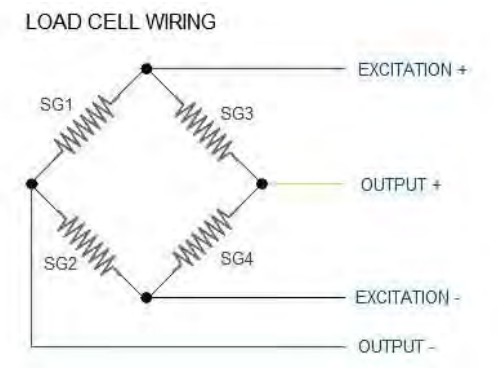
\includegraphics[width=0.35\textwidth]{./gambar/wheatstone_loadcell.png}
        \caption{Wheatstone Bridge Circuit on Load Cell\cite{rahman2018autonomous}.}
        \label{fig:Wheatstone_Bridge}
    \end{figure}
    
    \begin{equation}
      V_{\mathrm{out}} = V_{\mathrm{in}} \cdot \frac{R_2 \cdot R_3 - R_1 \cdot R_4}{(R_1 + R_2) \cdot (R_3 + R_4)}
      \label{eq:Wheatstone_Bridge}
    \end{equation}
    
    \hspace*{1em} Inside the Load Cell Sensor, the system is equipped with a Wheatstone Bridge circuit. The Wheatstone Bridge, as shown in Figure \ref{fig:Wheatstone_Bridge}, is a circuit used to measure resistance changes with high sensitivity \cite{rahman2018autonomous}. To measure the resistance changes, the Wheatstone Bridge equation is used as in Equation \ref{eq:Wheatstone_Bridge}. 

    \item \textit{Real Time Operating System} (RTOS)
    \label{subsec:rtos}

    \hspace*{1em} The Real-Time Operating System (RTOS) is an essential component in modern embedded systems. Its ability to effectively manage concurrent tasks allows the system to process data from various sensors, such as load cells, simultaneously, and control actuators with high precision \cite{sayyad2023real}. RTOS allows the system to perform multiple tasks simultaneously, prioritizing more important tasks \cite{digikey2021task}. This enables the robot to respond quickly to environmental changes, such as maintaining balance, and overall improves the performance and adaptability of robotics using embedded systems.

    \item PID Control System
    \label{subsec:sistemkontrolpid}

    \hspace*{1em} The use of a PID (Proportional-Integral-Derivative) control system is a common method used in servo motor control. This system helps maintain the balance and stability of the robot by correcting movements based on the error values generated from the difference between the actual position and the desired position. PID consists of three main components: proportional control (P), integral control (I), and differential control (D). Each of these components functions to correct errors in different ways.

    \hspace*{1em} The combination of these three components forms an effective PID control in maintaining the balance and stability of the robot. Proper adjustment of the $K_p$, $K_i$, and $K_d$ parameters is crucial to ensure the system performs optimally and responsively.

    \begin{equation}
      \mathrm{Correction} = K_p \cdot \mathrm{error} + K_i \cdot \int_{0}^{t} \mathrm{error} \cdot dt + K_d \cdot \frac{d\mathrm{error}}{dt}
    \end{equation}

    \item Center of Pressure
    \label{subsec:pusattekanan}

    \hspace*{1em} The center of pressure is the point where all forces are concentrated without any torque moment \cite{hawley2016external}. In this center of pressure, several pressures are calculated based on the cross-sectional area to obtain the position of the center of pressure. The Center of Pressure is related to the balance of the robot, especially at the center of gravity \cite{arifin2017implementasi}.

    \begin{equation}
      X_{\mathrm{cop}} = X_0 + \frac{(F2 + F4) \cdot dx}{F1 + F2 + F3 + F4}
      \label{eq:COP_X_1}
    \end{equation}

    \begin{equation}
      Y_{\mathrm{cop}} = Y_0 + \frac{(F1 + F2) \cdot dy}{F1 + F2 + F3 + F4}
      \label{eq:COP_Y_1}
    \end{equation}


    \begin{figure} [h] \centering
      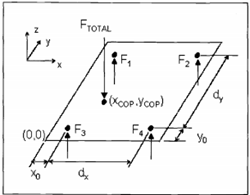
\includegraphics[width=0.3\textwidth]{gambar/Konsep_Letak.png}
      \caption{Concept of Pressure Sensor Placement\cite{resna2005}.}
      \label{fig:Konsep_Letak}
    \end{figure}

    \hspace*{1em} Figure \ref{fig:Konsep_Letak} shows the concept of pressure sensor placement. From this concept, the center of pressure can be calculated using Equations \ref{eq:COP_X_1} and \ref{eq:COP_Y_1}.
\end{enumerate}

\newpage
\section{Design and Implementation}
\label{sec:designandimplementation}

\begin{enumerate}[label=\Alph*.]
    \item System Block Diagram
    \label{subsec:systemblockdiagram}

    \hspace*{1em} The designed system has several main components: the sensor part, the control part, the mechanical system part, and the motion data part.

    \begin{figure} [h] \centering
        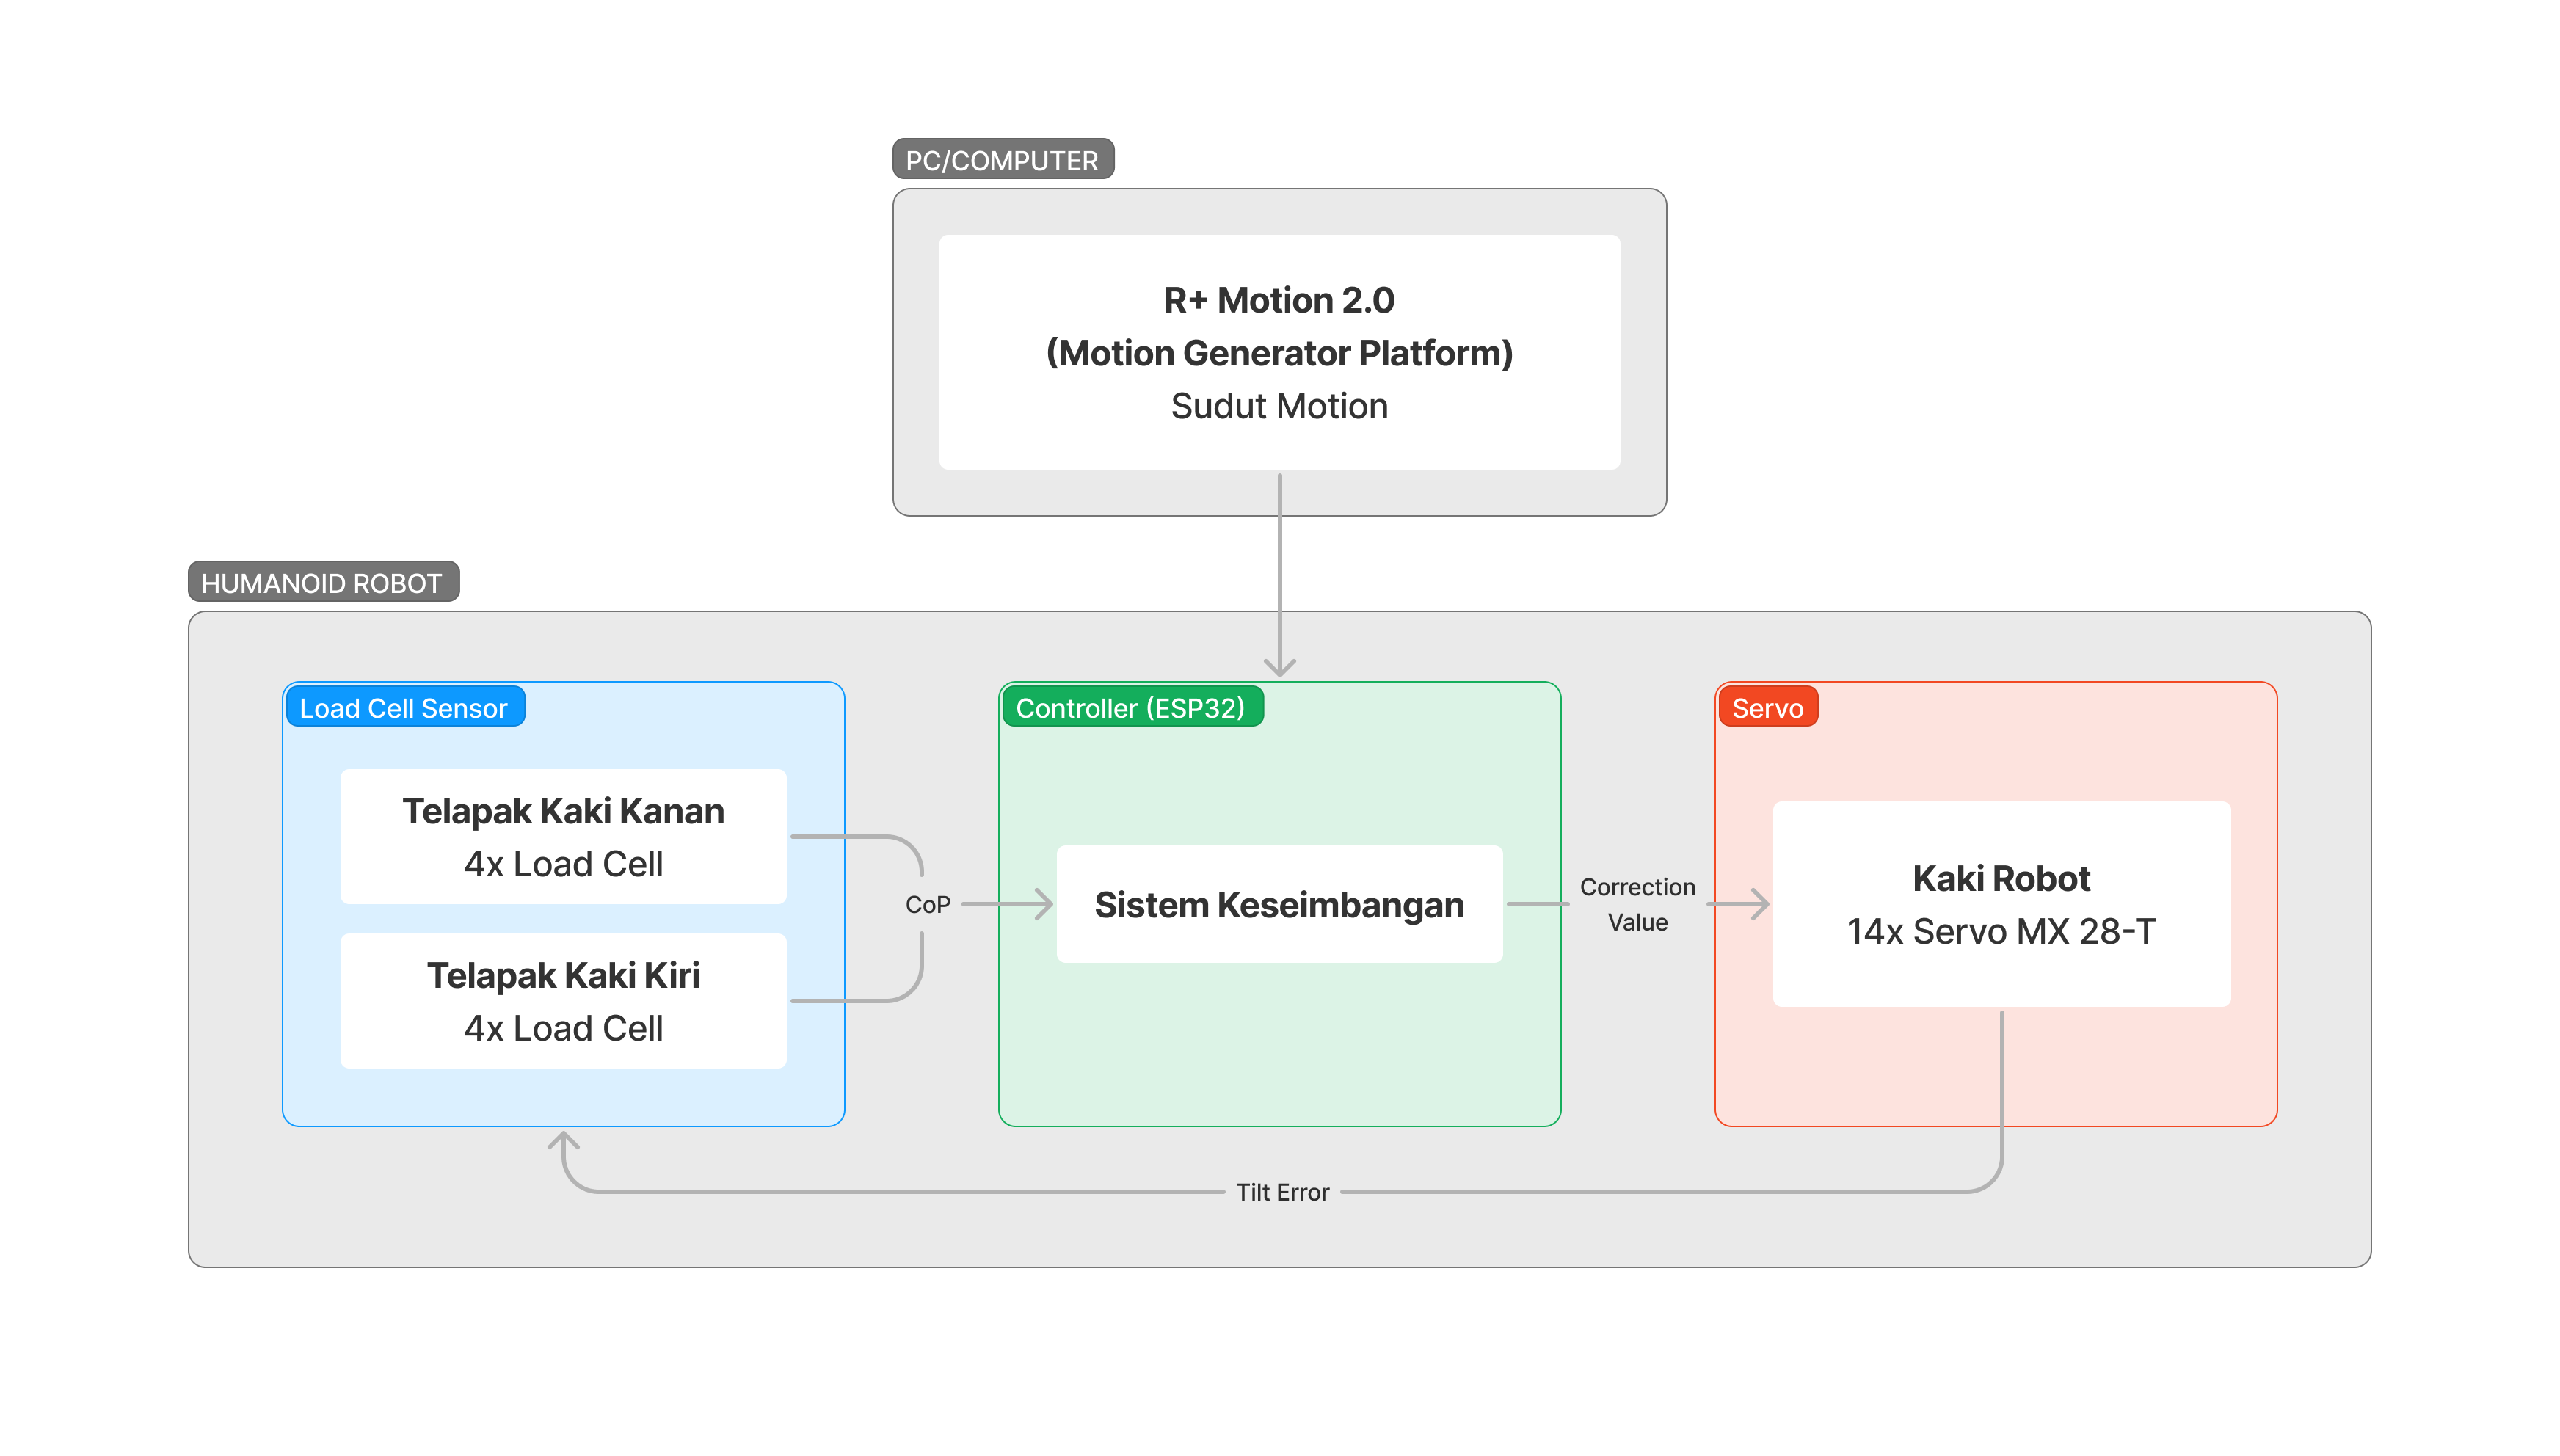
\includegraphics[width=0.45\textwidth]{gambar/Diagram_Sistem.png}
        \caption{Overall System Diagram}
        \label{fig:Diagram_Sistem}
    \end{figure}
    
    \hspace*{1em} The sensor part includes load cells mounted on each foot of the robot. These load cells detect the load or pressure on the robot's feet. The control part involves a microcontroller responsible for processing data from the sensors and controlling the robot's movements. The mechanical system part includes the robot's frame consisting of various servos used to move the robot. The motion data part stores pre-designed movements in the microcontroller's file system. This data consists of several frames containing an array of target positions for each servo along with the time required to reach those positions. The system diagram can be seen in Figure \ref{fig:Diagram_Sistem}.

    \item Mechanical System
    \label{subsec:mechanicalsystem}

    \hspace*{1em} The design of the humanoid robot body includes 29 degrees of freedom. The upper body uses 15 XL-320 type servos, while the lower body uses 14 MX-28 type servos. The detailed design, dimensions, and servo ID naming on the robot can be seen in Figure \ref{fig:Desain_Mekanik}. 

    \begin{figure} [h] \centering
      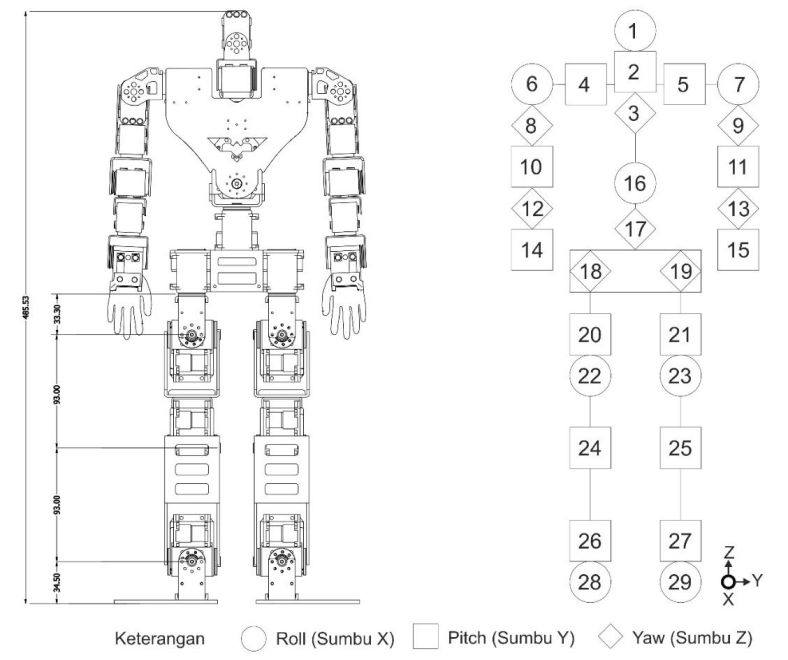
\includegraphics[width=0.35\textwidth]{gambar/Desain_Mekanik.png}
      \caption{Mechanical Design of the Robot and Servo ID Naming}
      \label{fig:Desain_Mekanik}
    \end{figure}

    \item Electronic System
    \label{subsec:electronicsystem}

    \hspace*{1em} The hardware system in this research is explained through the block diagram shown in Figure \ref{fig:Diagram_Elektronik}. This system uses an embedded system consisting of ESP32 and ESP32-C3 microcontrollers. The embedded system was chosen because the robot developed in this research is an improvement from previous research conducted by Fahd (2018)\cite{fahd}.

    \begin{figure} [h] \centering
      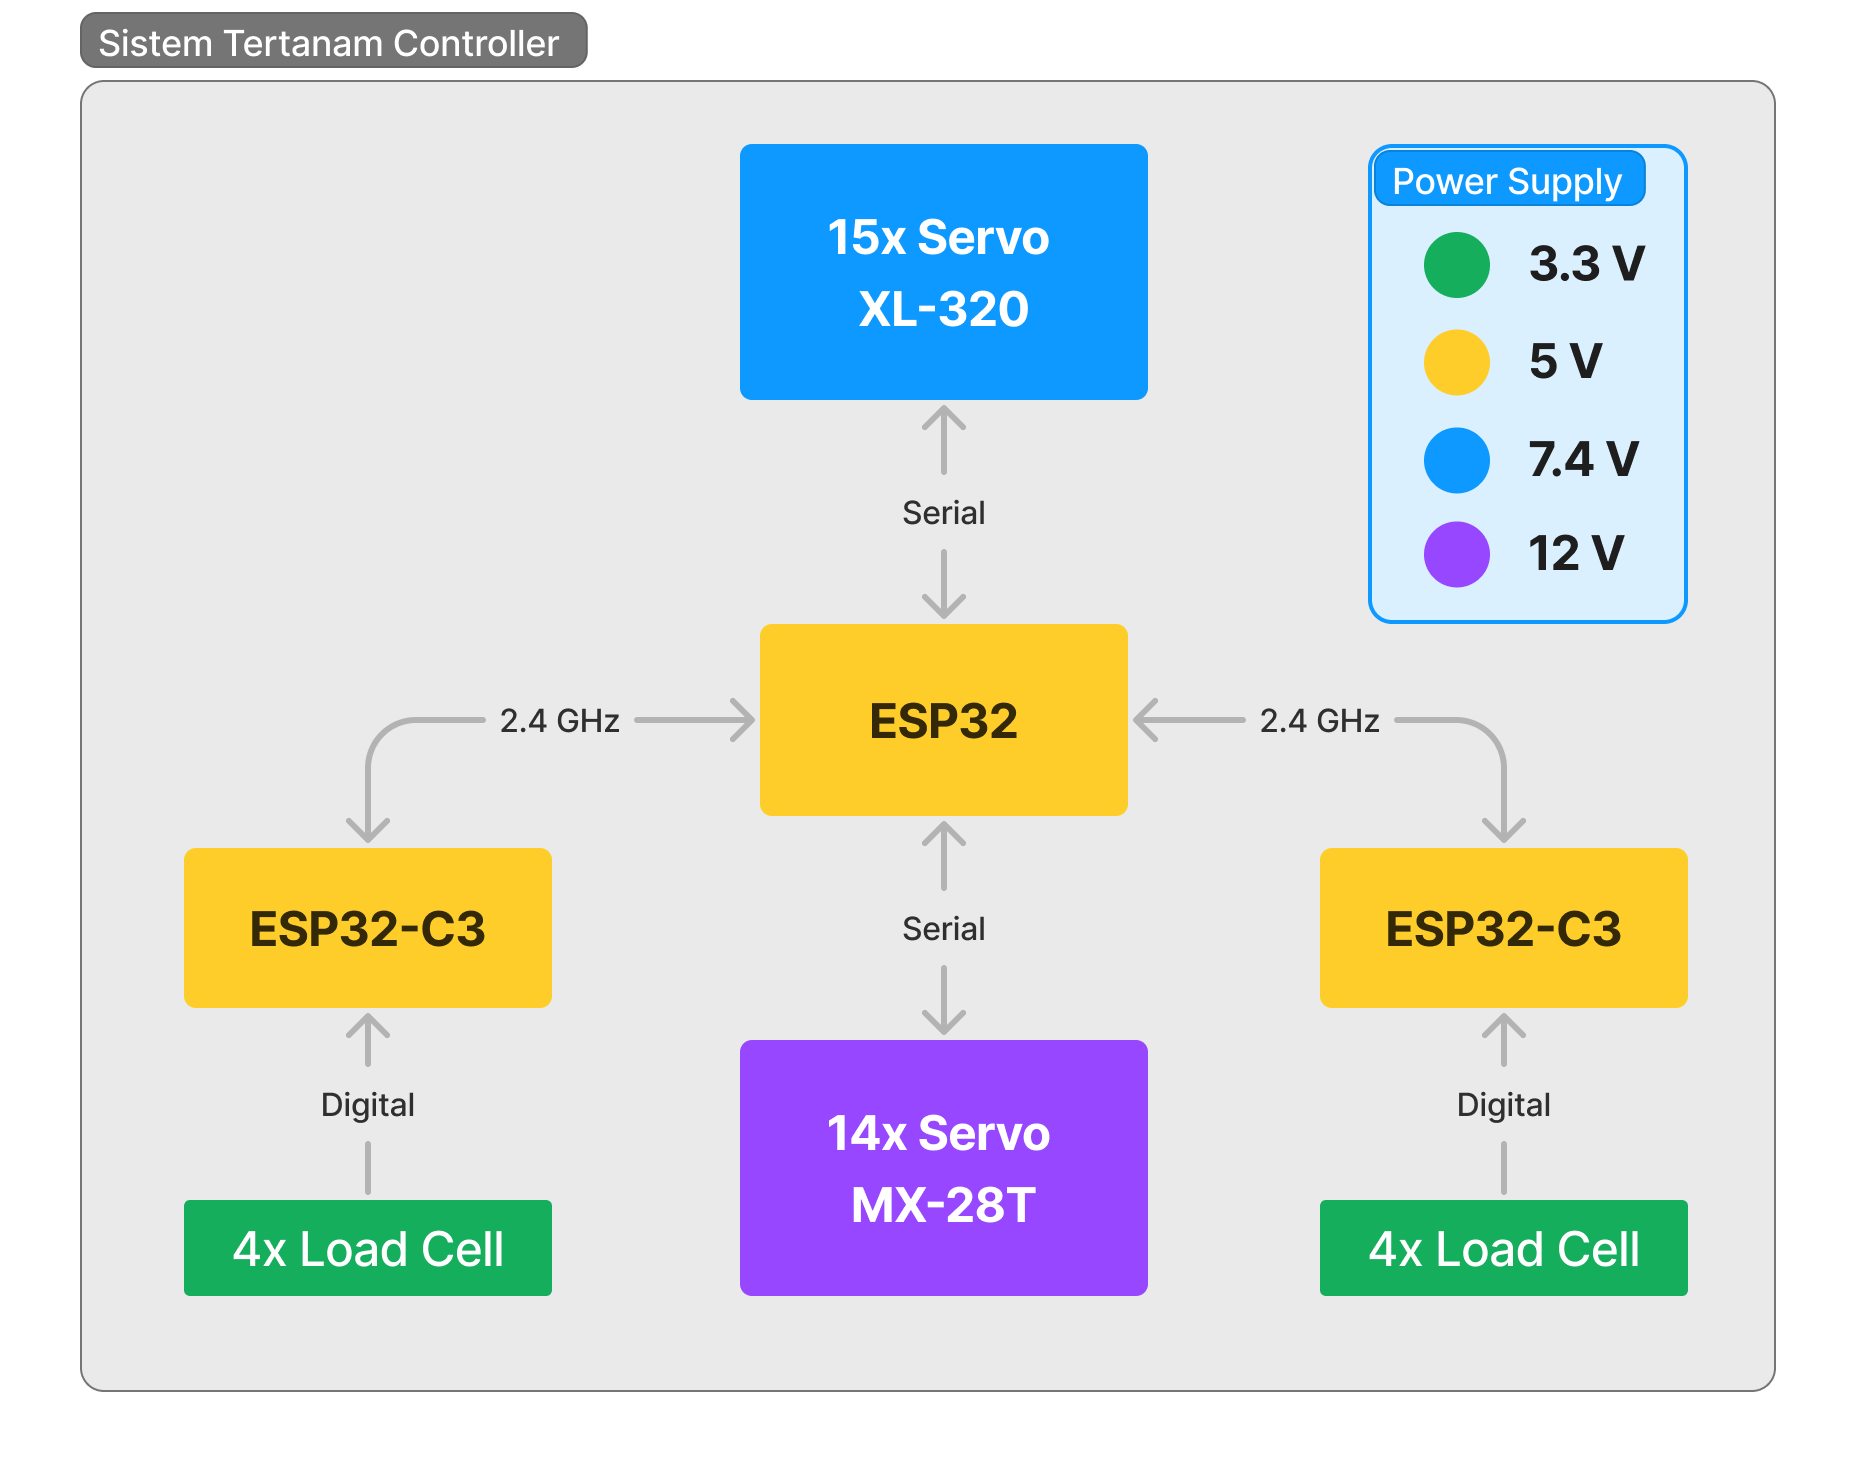
\includegraphics[width=0.4\textwidth]{gambar/Diagram_Elektronik.png}
      \caption{Electronic and Communication Diagram Between Components}
      \label{fig:Diagram_Elektronik}
    \end{figure}

    \hspace*{1em} ESP32-C3 is used for data acquisition from the load cell and sends it to the ESP32. ESP32-C3 has the same Wi-Fi capability as ESP32, allowing wireless communication between the two microcontrollers. ESP32-C3 also has a smaller dimension, making it easier to be placed on the robot's foot.

    \item Foot Design of the Robot
    \label{subsec:desaignsystemloadcell}

    \hspace*{1em} Each robot foot is equipped with 4 load cells mounted at the ends of the foot. Each load cell detects pressure, allowing the system to determine the center of pressure on the robot's foot. The design of the robot foot can be seen in Figure \ref{fig:Desain_Kaki}.
    
    \begin{figure} [h] \centering
      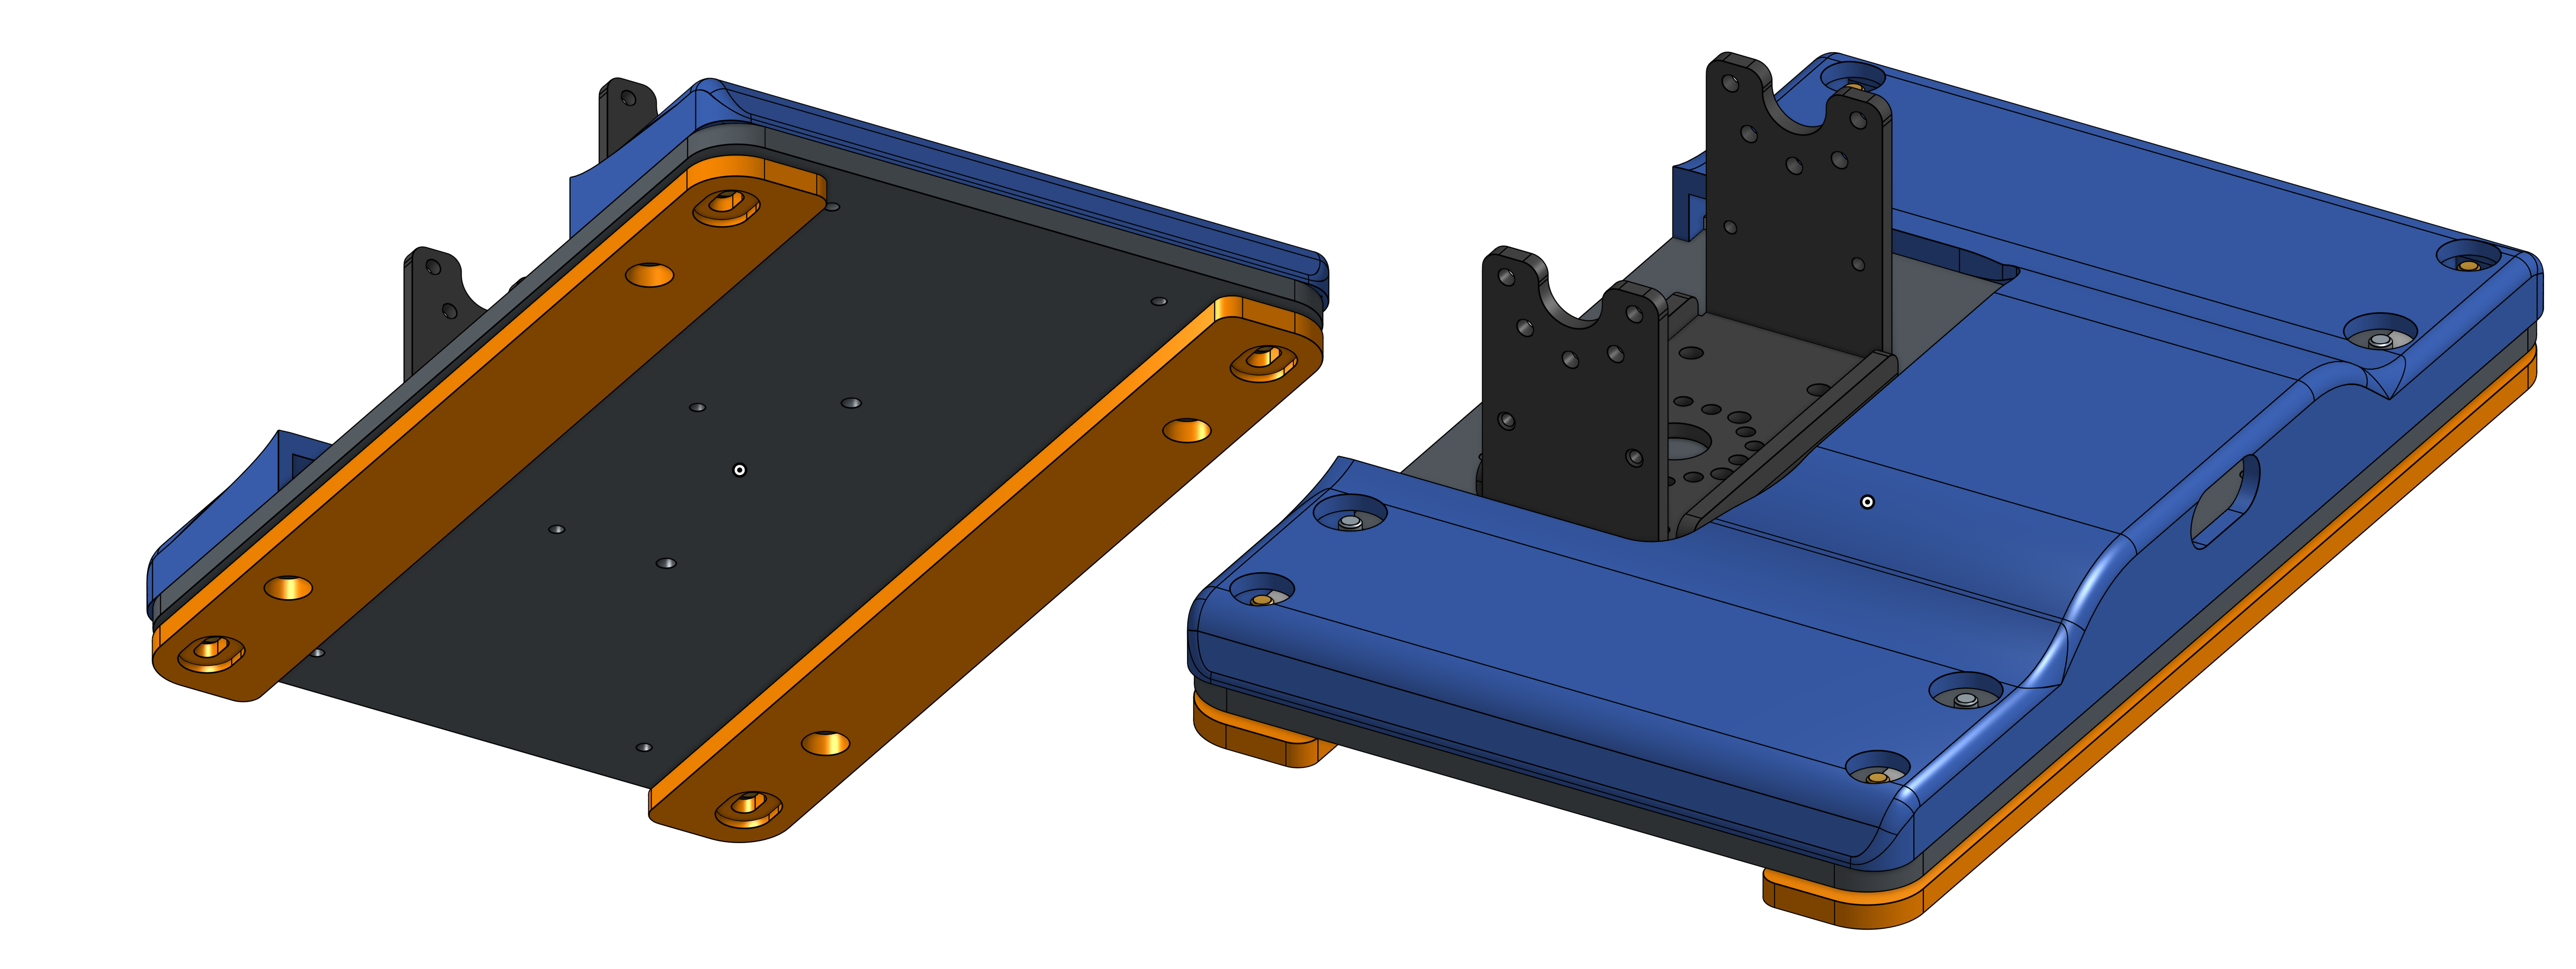
\includegraphics[width=0.4\textwidth]{gambar/Desain_Kaki.png}
      \caption{Overall Design of the Robot Foot}
      \label{fig:Desain_Kaki}
    \end{figure}

    \hspace*{1em} In Figure \ref{fig:Desain_Kaki}, it is shown that each load cell is placed at the end of the robot's foot. The load cells are connected to a microcontroller located inside the robot's foot. For the electronics part, a closure made from 3D print is provided to protect the components from damage. For the mechanical part, the load cell sensors are equipped with pads that serve as pressure points for the load cells and also provide anti-slip to prevent slipping.

    \item Load Cell Coefficient Configuration
    \label{subsec:configurationcoefficient}

    \hspace*{1em} Before the load cells can be used, calibration is necessary to measure the load cell coefficients by adjusting parameters such as scaling and offset values. To facilitate configuration, a graphical user interface (GUI) application was created, which is user-friendly and can be accessed through a browser. This GUI has a control menu for accessing functions and settings, and displays the center of pressure to visualize the impact of parameter changes on the system. Figure \ref{fig:Preview_Aplikasi} shows the configuration application interface, including the control menu and center of pressure display. This application will save configuration data to the EEPROM memory of the microcontroller, so the data remains stored even when the microcontroller is turned off.

    \begin{figure} [h] \centering
      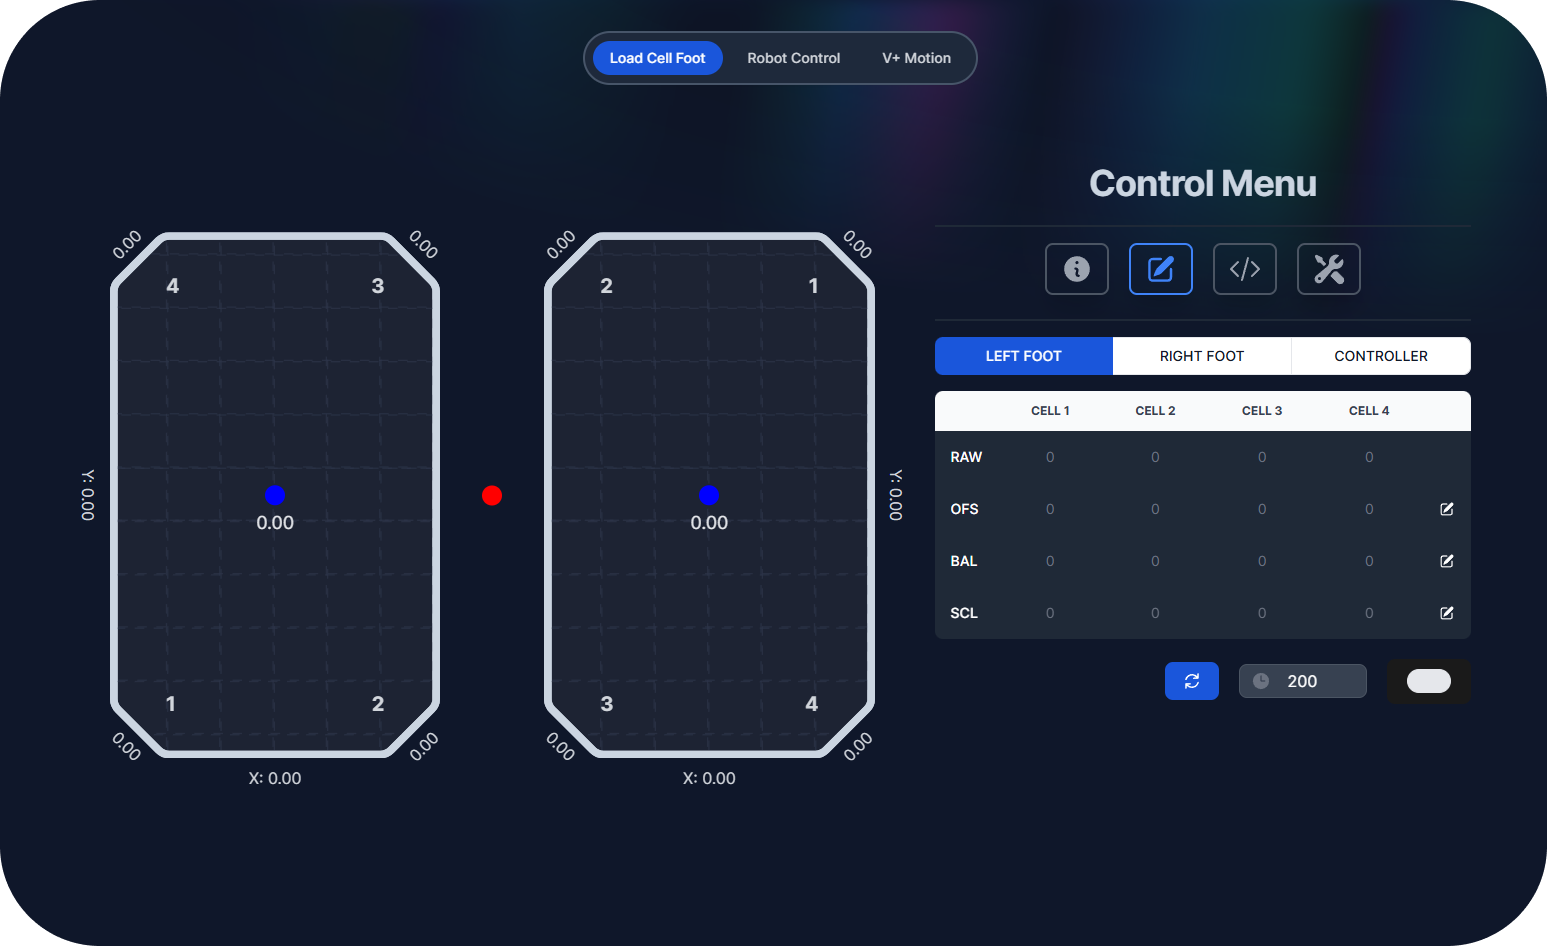
\includegraphics[width=0.4\textwidth]{gambar/preview_aplikasi.png}
      \caption{Application Used for Load Cell Configuration}
      \label{fig:Preview_Aplikasi}
    \end{figure}

    \item Center of Pressure Calculation for the Robot
    \label{subsec:pressurecentercalculation}

    \hspace*{1em} The center of pressure on the robot is calculated by combining data from both robot feet. The main microcontroller will communicate with the microcontrollers on the left and right feet to obtain the center of pressure and total pressure data. This data is then used to determine the position of the center of pressure relative to the robot. The calculation of the center of pressure position on the robot is done as shown in equations \ref{eq:Total_Force_Robot}, \ref{eq:COP_X_Robot}, and \ref{eq:COP_Y_Robot}.
    
    \begin{figure} [h] \centering
      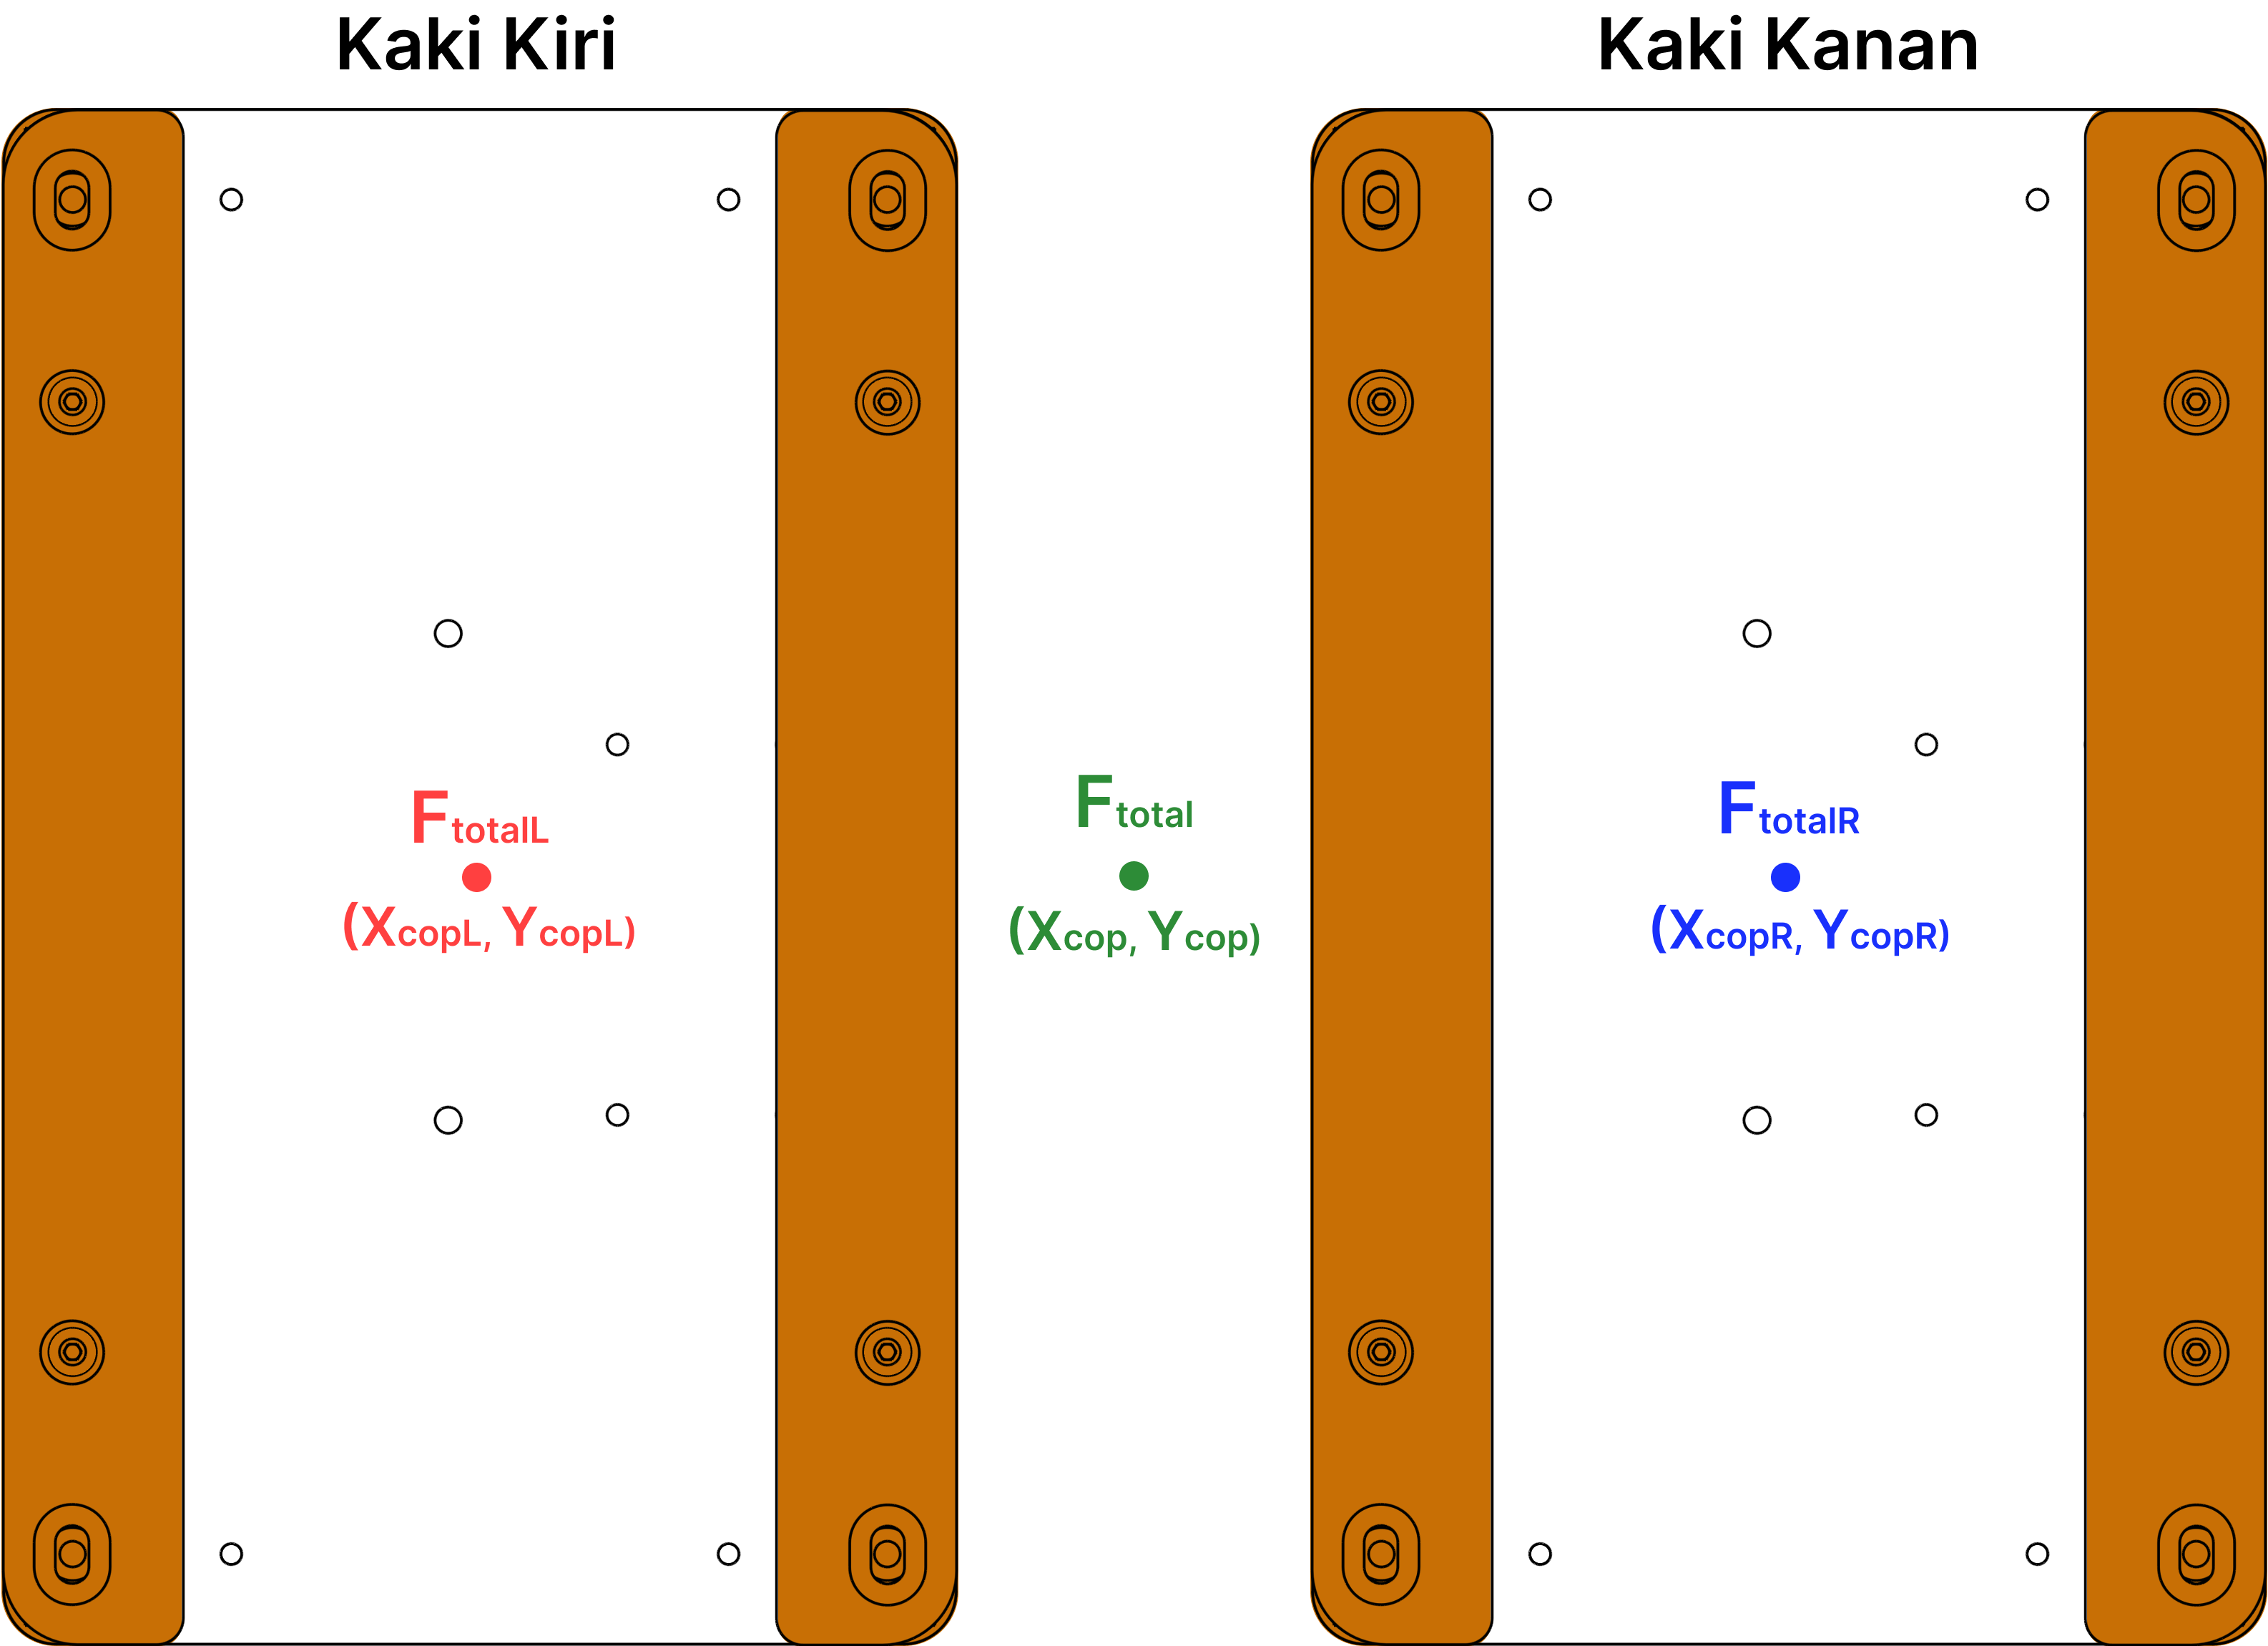
\includegraphics[width=0.4\textwidth]{gambar/COP_Robot.png}
      \caption{Center of Pressure on the Robot (Green), Center of Pressure on the Left Foot (Red), and Center of Pressure on the Right Foot (Blue)}
      \label{fig:COP_Robot}
    \end{figure}

    \begin{equation}
      F_{\mathrm{total}} = F_{\mathrm{totalL}} + F_{\mathrm{totalR}}
      \label{eq:Total_Force_Robot}
    \end{equation}

    \begin{equation}
      X_{\mathrm{cop}} = \frac{F_{\mathrm{totalL}} \cdot X_{\mathrm{copL}} + F_{\mathrm{totalR}} \cdot X_{\mathrm{copR}}}{F_{\mathrm{total}}}
      \label{eq:COP_X_Robot}
    \end{equation}

    \begin{equation}
      Y_{\mathrm{cop}} = \frac{F_{\mathrm{totalL}} \cdot Y_{\mathrm{copL}} + F_{\mathrm{totalR}} \cdot Y_{\mathrm{copR}}}{F_{\mathrm{total}}}
      \label{eq:COP_Y_Robot}
    \end{equation}

    \hspace*{1em} The center of pressure data in this study will use a scale. As shown in Figure \ref{fig:COP_Robot}, the Y-axis has a scale from -1 to 1. The upper limit is represented by the value 1, while the lower limit is represented by the value -1. The X-axis has a scale from -2 to 2, with the right limit represented by the value 2 and the left limit represented by the value -2. For the X-axis, when the robot's weight is supported on one foot, the center of pressure value will be positive or negative depending on the position of the supporting foot. When the robot is lifted, the center of pressure value will be at (0,0), which is in the middle of the foot.

    \item PID Control System Algorithm
    \label{subsec:algoritmakontrolpid}

    \hspace*{1em} In this research, there are two PID controls, namely the Pitch PID control and the Roll PID control. In the Pitch PID control, the input is the position value of the center of pressure on the Y-axis. Meanwhile, in the Roll PID control, the input is the position value of the center of pressure on the X-axis. For the Pitch and Roll PID control setpoints, the values found from the previous center of pressure data collection are used. In Equation \ref{eq:Error_PID}, the error value is obtained from the difference between the current center of pressure position and the setpoint. Then, in Equation \ref{eq:Koreksi_PID}, the error value is used to calculate the correction value that will be used to adjust the servo position as compensation.

    \begin{equation}
      \mathrm{e} = COP_{\mathrm{error}} = COP_{\mathrm{set}} - COP_{\mathrm{input}}
      \label{eq:Error_PID}
    \end{equation}

    \begin{equation}
      \theta_\mathrm{e} = \mathrm{Kp} \cdot \mathrm{e} + \mathrm{Ki} \cdot \int \mathrm{e} + \mathrm{Kd} \cdot \frac{\mathrm{de}}{\mathrm{dt}}
      \label{eq:Koreksi_PID}
    \end{equation}
    
    \hspace*{1em} In the flowchart in Figure \ref{fig:Flow_Kontrol}, the system response stages to the error caused by the difference between the desired and actual center of pressure positions are shown. First, the PID values are set according to the system characteristics, then the setpoint is set according to the desired center of pressure position. The error is calculated using Equation \ref{eq:Error_PID}. This error value is used to calculate the correction using Equation \ref{eq:Koreksi_PID}. The robot will perform movements to maintain balance based on the corrections generated by the PID control, which continues until the robot's motion is complete.

    \begin{figure} [h] \centering
      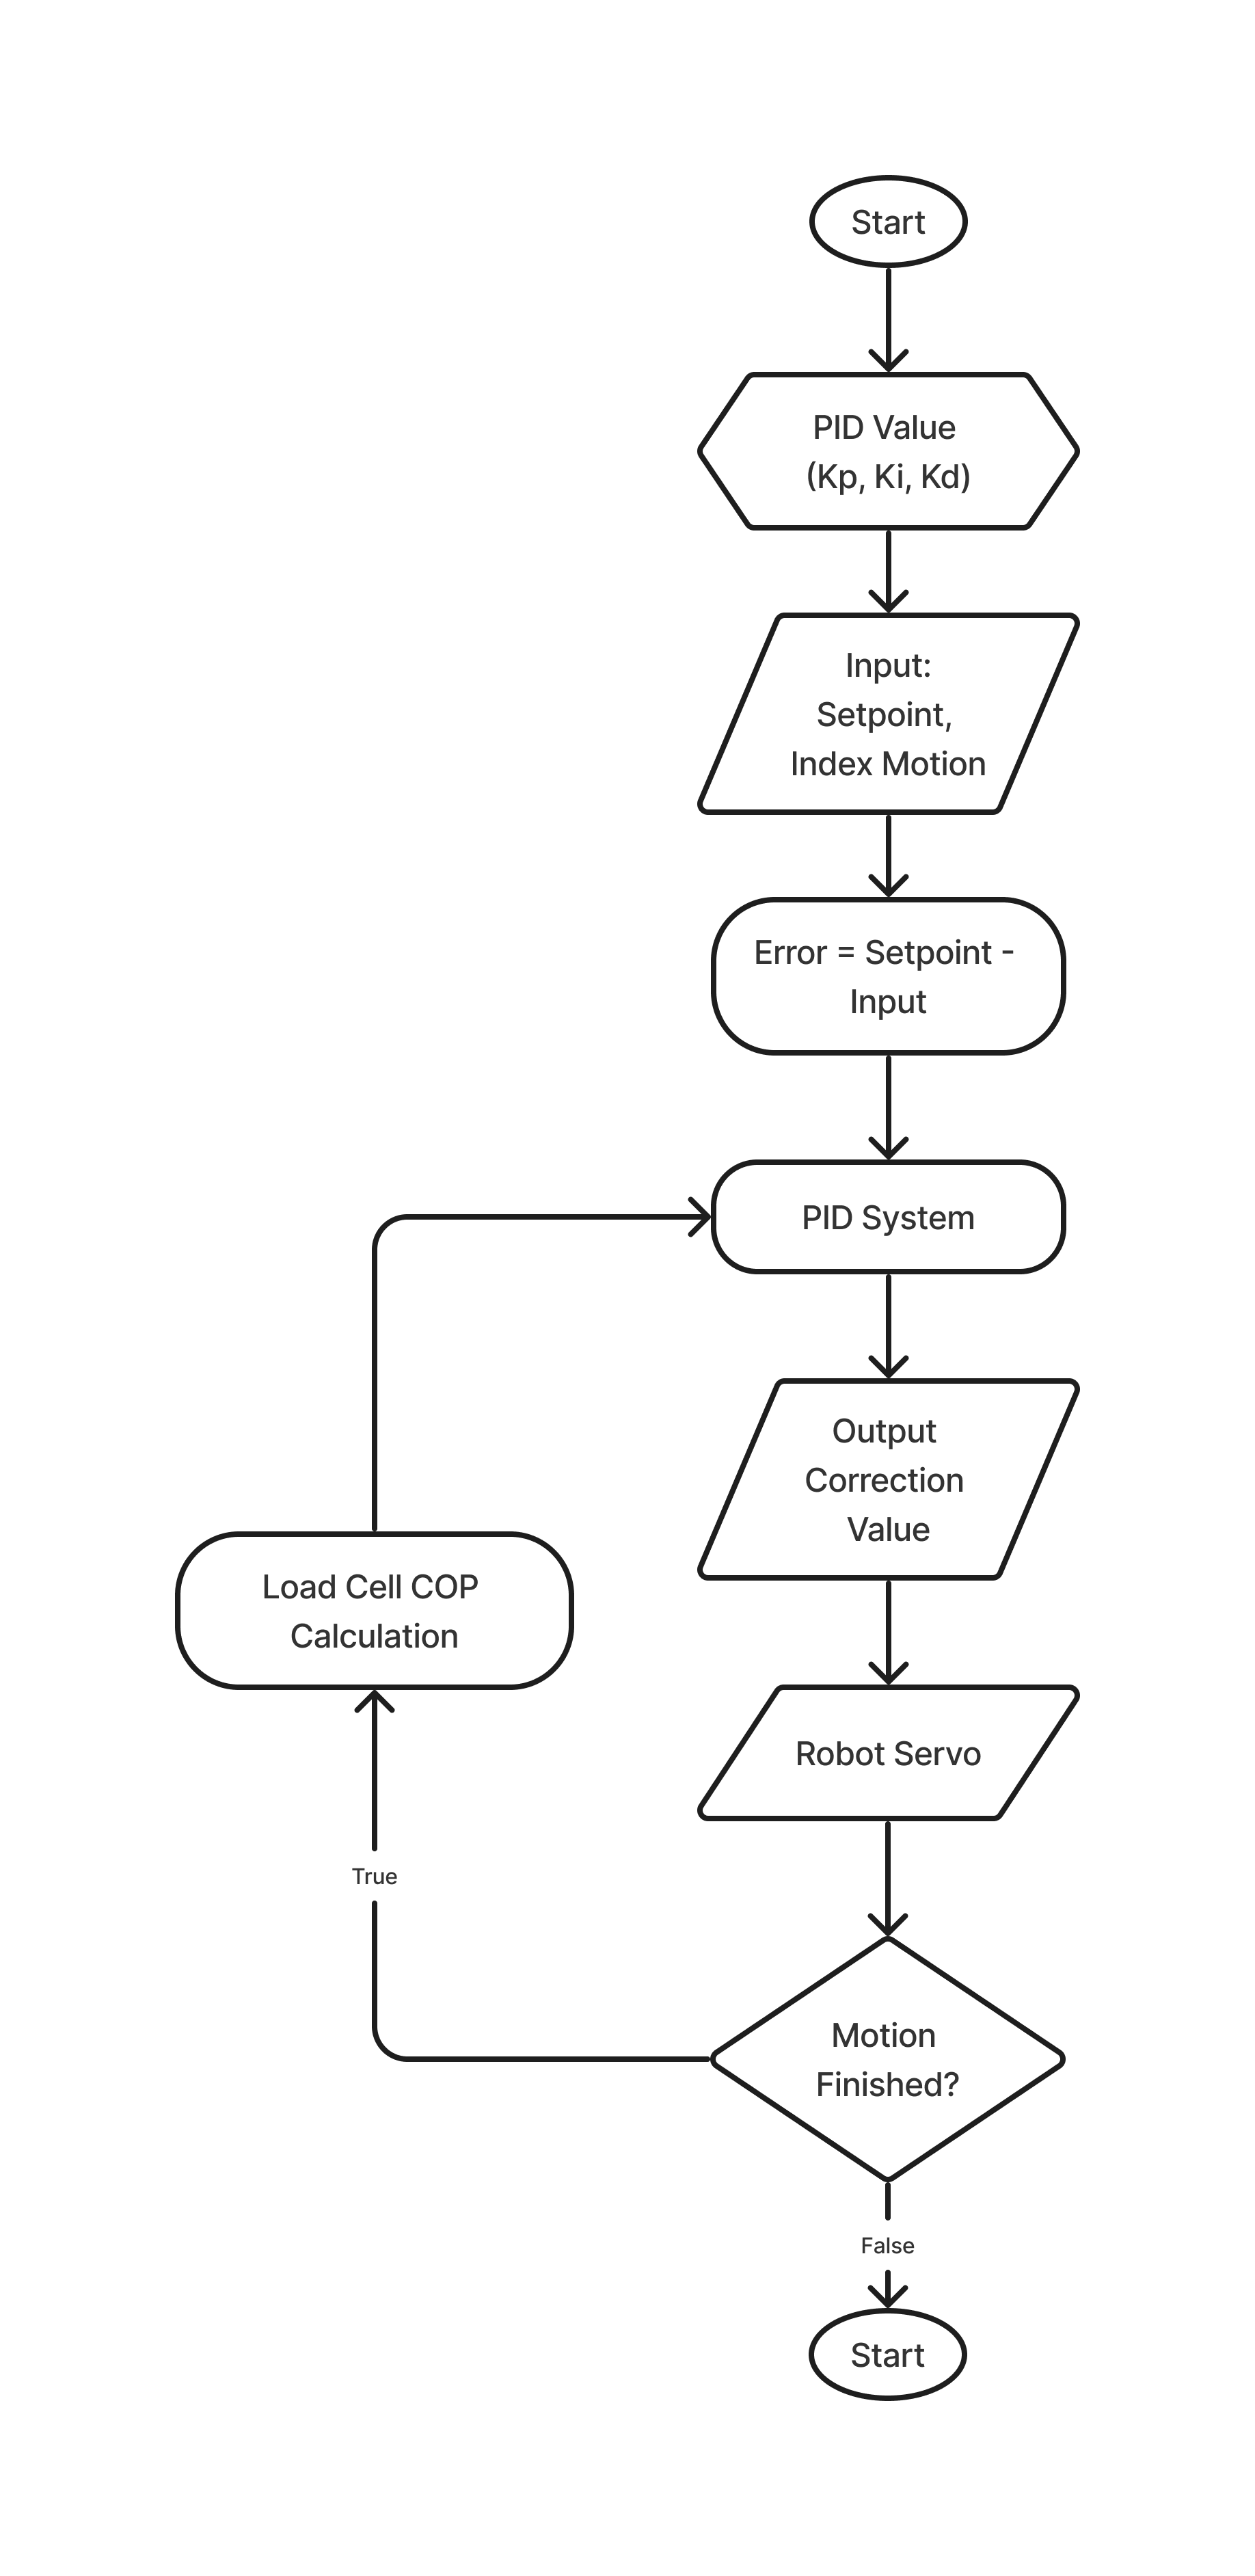
\includegraphics[width=0.38\textwidth]{gambar/Flow_Kontrol.png}
      \caption{PID Control System Flowchart When the Robot is in Motion}
      \label{fig:Flow_Kontrol}
    \end{figure}

    \begin{figure} [h] \centering
      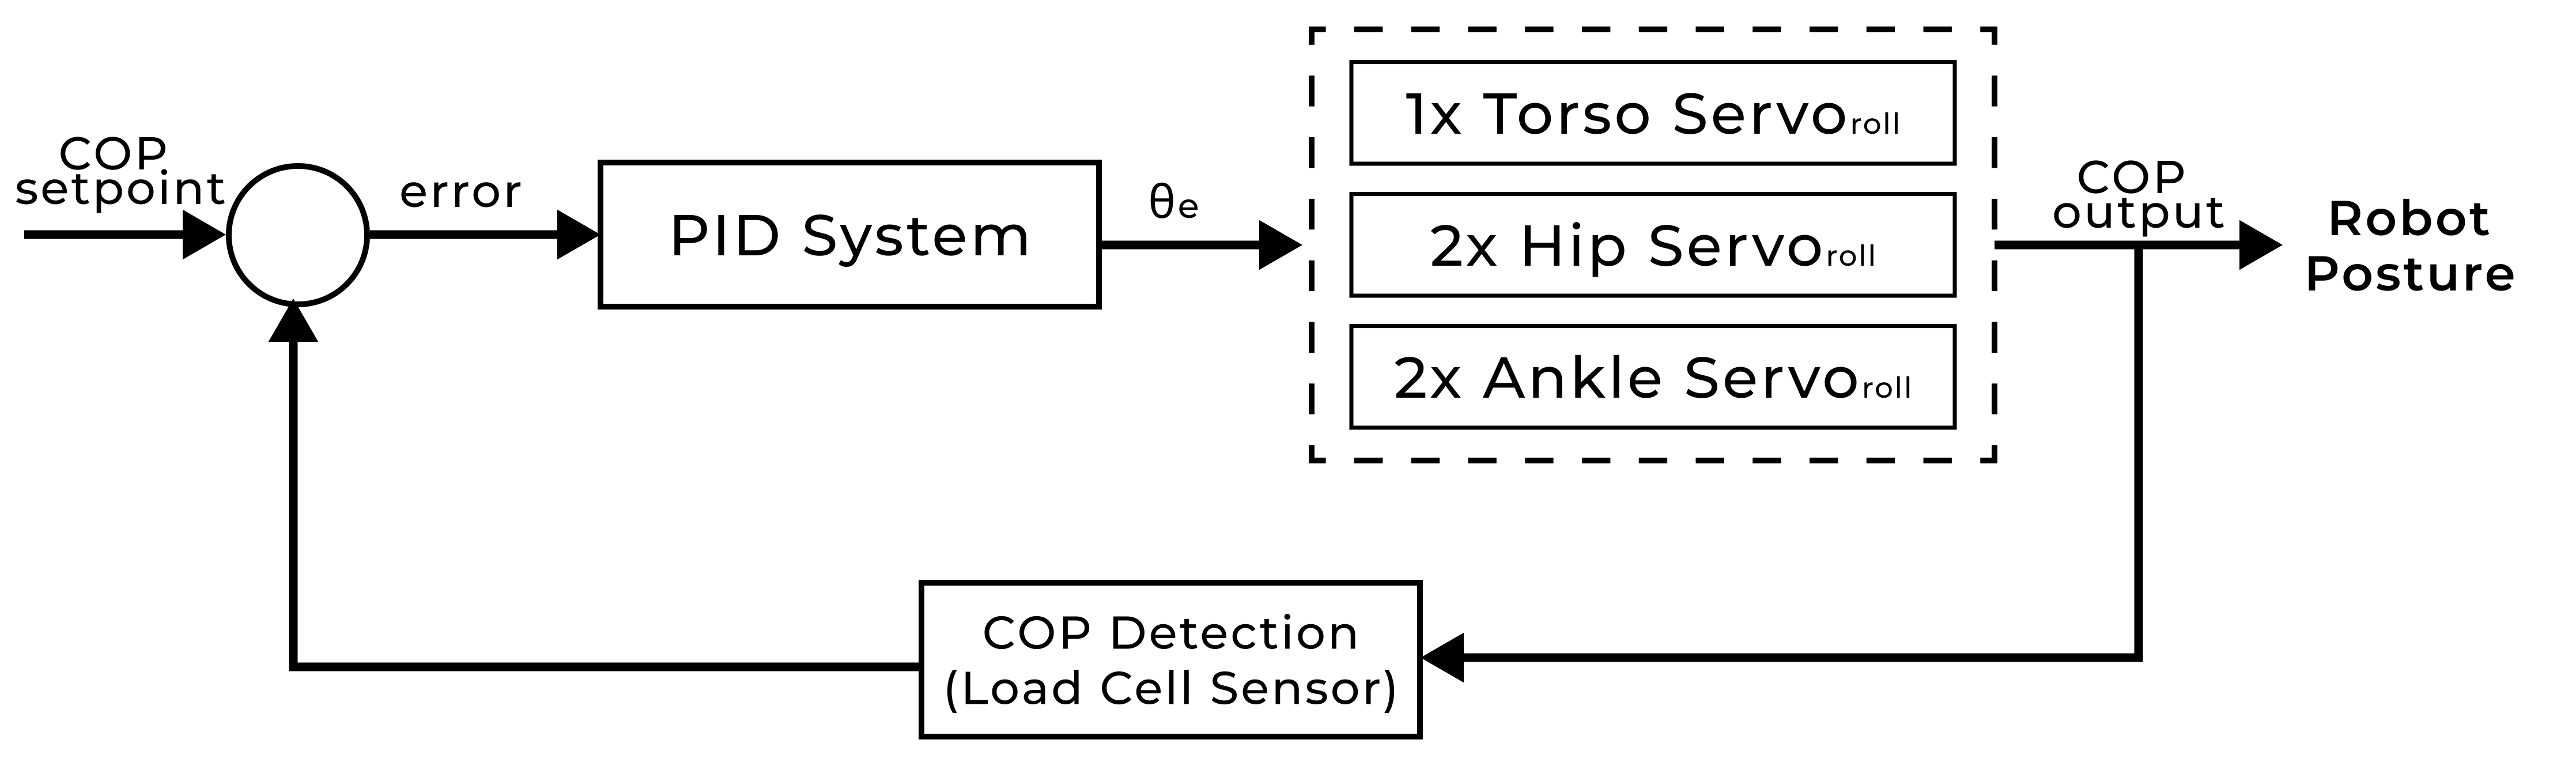
\includegraphics[width=0.4\textwidth]{gambar/pid_diagram.png}
      \caption{PID Control System Diagram}
      \label{fig:Control_System}
    \end{figure}

    \hspace*{1em} Figure \ref{fig:Control_System} shows the control system diagram consisting of three main blocks: the PID block, the servo block as compensation, and the center of pressure block. The PID System block calculates the correction value using Equation \ref{eq:Koreksi_PID}. The error value is obtained from the difference between $COP_{setpoint}$ and $COP_{input}$. This correction value is used to adjust the servo position in the servo block as compensation using 5 servos that control the robot's roll position. The center of pressure block calculates the center of pressure position on the robot's foot and provides this data as input to the PID control.

    \item Servo Settings as Compensation
    \label{subsec:servosettings}

    \hspace*{1em} In this research, the servos used to maintain balance are the servos that control the robot's roll position. These servos are located on the torso, hip, and ankle. By adjusting several servo angles, the robot can make the necessary adjustments to maintain balance when moving or standing on uneven surfaces. There are five servos used, consisting of one servo on the torso (ID 1), two servos on each hip (ID 4 and ID 5), and two servos on each ankle (ID 13 and ID 14). The servo settings as compensation can be seen in Figure \ref{fig:Controlled_Servo}, indicated by the blue-colored servos.

    \begin{figure} [h] \centering
      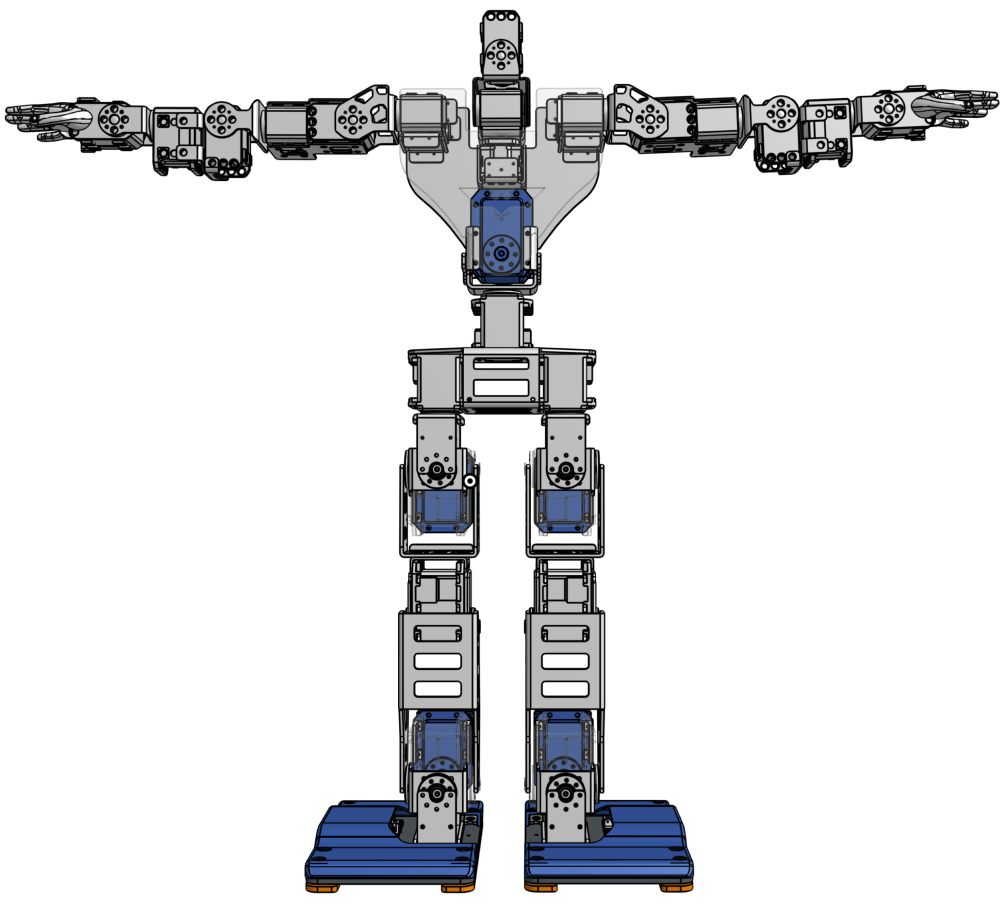
\includegraphics[width=0.4\textwidth]{gambar/controlled_servo.png}
      \caption{Servo Settings as Compensation Indicated by Blue Color}
      \label{fig:Controlled_Servo}
    \end{figure}

    \begin{equation}
      \theta_{\mathrm{torso}} = \theta_{\mathrm{torso}} + (\theta_\mathrm{e}{\mathrm{roll}} \cdot 0.8)
      \label{eq:Koreksi_Torso}
    \end{equation}

    \begin{equation}
      \theta_{\mathrm{hip}} = \theta_{\mathrm{hip}} + (\theta_\mathrm{e}{\mathrm{roll}} \cdot 1)
      \label{eq:Koreksi_Hip}
    \end{equation}

    \begin{equation}
      \theta_{\mathrm{ankle}} = \theta_{\mathrm{ankle}} + (\theta_\mathrm{e}{\mathrm{roll}} \cdot 0.4)
      \label{eq:Koreksi_Ankle}
    \end{equation}

    \hspace*{1em} In Equation \ref{eq:Koreksi_Torso}, the correction value is used to adjust the servo position on the torso with a factor of 0.8. In Equation \ref{eq:Koreksi_Hip}, the correction value is used to adjust the servo position on the hip with a factor of 1. In Equation \ref{eq:Koreksi_Ankle}, the correction value is used to adjust the servo position on the ankle with a factor of 0.4. The scaling of the correction value on the servo is determined by trial and error, considering the impact on each part of the robot's body and the specifications of the servos used.

\hspace*{1em} 
\end{enumerate}
\section{Results and Discussion}
\label{sec:resultsanddiscussion}

Testing and analysis were conducted on the previously designed and implemented systems. The tests included Load Cell Sensor testing on the Robot and the Robot Balance System.

\begin{enumerate}[label=\Alph*.]

    \item Characterization Testing on Each Load Cell Sensor
    \label{subsec:results-discussion-characterization}

        \hspace*{1em} Calibration tests for the load cell sensors were conducted using five reference mass weights (50g, 100g, 200g, 500g, and 1000g) to determine the gradient coefficient and tare weight constant. The load cells were connected in two groups: Load Cell 1 and 4, and Load Cell 2 and 3.

        \begin{table}[h]
            \centering
            \caption{First Load Cell Characterization Results}
            \begin{tabular}{|c|c|c|}
                \hline
                \textbf{Actual Weight (g)} & \textbf{Load Cell 1 Reading (g)} & \textbf{Error (g)} \\
                \hline
                50    & 50    & 0   \\
                100   & 101   & 1   \\
                200   & 202   & 2   \\
                500   & 505   & 5   \\
                1000  & 1004  & 4   \\
                \hline
            \end{tabular}
            \label{tab:Calibration_Load_Cell_1}
        \end{table}

        \begin{table}[h]
            \centering
            \caption{Second Load Cell Characterization Results}
            \begin{tabular}{|c|c|c|}
                \hline
                \textbf{Actual Weight (g)} & \textbf{Load Cell 2 Reading (g)} & \textbf{Error (g)} \\
                \hline
                50        & 50        & 0   \\
                100       & 100       & 0   \\
                200       & 200       & 0   \\
                500       & 500       & 0   \\
                1000      & 994       & 6   \\           
                \hline
        \end{tabular}
        \label{tab:Calibration_Load_Cell_2}
        \end{table}

        \begin{table}[h]
            \centering
            \caption{Third Load Cell Characterization Results}
            \begin{tabular}{|c|c|c|}
                \hline
                \textbf{Actual Weight (g)} & \textbf{Load Cell 3 Reading (g)} & \textbf{Error (g)} \\
                \hline
                50        & 50        & 0    \\    
                100       & 103       & 3    \\    
                200       & 203       & 3    \\    
                500       & 494       & 6    \\    
                1000      & 981       & 19   \\               
                \hline
        \end{tabular}
        \label{tab:Calibration_Load_Cell_3}
        \end{table}

        \begin{table}[h]
            \centering
            \caption{Fourth Load Cell Characterization Results}
            \begin{tabular}{|c|c|c|}
                \hline
                \textbf{Actual Weight (g)} & \textbf{Load Cell 4 Reading (g)} & \textbf{Error (g)} \\
                \hline
                50        & 50        & 0   \\     
                100       & 97        & 3   \\     
                200       & 204       & 4   \\     
                500       & 500       & 0   \\     
                1000      & 1003      & 3   \\                
                \hline
        \end{tabular}
        \label{tab:Calibration_Load_Cell_4}
        \end{table}
    
        
        \hspace*{1em} The digital readings from the load cells were converted into actual mass using calibration equations, and errors were measured by comparing the results with the actual masses. The measurement results showed errors ranging from 0 to 20 grams. Although not entirely linear, the calibration equations used were sufficiently accurate with an error tolerance of 5%.

    \item Pressure Testing on Foot Soles
    \label{subsec:results-discussion-pressure}

        \hspace*{1em} This test was conducted to obtain pressure data generated by the right and left feet when equally loaded. The pressure data generated by the right and left feet can be seen in Table \ref{tab:left_foot_weight_measurement} and Table \ref{tab:right_foot_weight_measurement}.

        \begin{table}[h!]
            \centering
            \caption{Pressure Reading Table for the Left Foot}
            \begin{tabular}{|c|c|c|}
                \hline
                \textbf{Actual Weight (g)} & \textbf{Reading (g)} & \textbf{Error (g)} \\
                \hline
                50    & 52    & 2   \\
                100   & 110   & 10  \\
                200   & 220   & 20  \\
                300   & 304   & 4   \\
                500   & 512   & 12  \\
                700   & 701   & 1   \\
                1000  & 1050  & 50  \\
                1300  & 1325  & 25  \\
                1500  & 1512  & 12  \\
                1800  & 1788  & 12  \\
                \hline
                \textbf{Average Error (g)} & \multicolumn{2}{c|}{\textbf{14.8}} \\
                \hline
            \end{tabular}
            \label{tab:left_foot_weight_measurement}
        \end{table}

        \begin{table}[h!]
            \centering
            \caption{Pressure Reading Table for the Right Foot}
            \begin{tabular}{|c|c|c|}
                \hline
                \textbf{Actual Weight (g)} & \textbf{Reading (g)} & \textbf{Error (g)} \\
                \hline
                50    & 46    & 4    \\
                100   & 98    & 2    \\
                200   & 215   & 15   \\
                300   & 325   & 25   \\
                500   & 505   & 5    \\
                700   & 722   & 22   \\
                1000  & 1025  & 25   \\
                1300  & 1347  & 47   \\
                1500  & 1500  & 0    \\
                1800  & 1819  & 19   \\
                \hline
                \textbf{Average Error (g)} & \multicolumn{2}{c|}{\textbf{16.4}} \\
                \hline
            \end{tabular}
            \label{tab:right_foot_weight_measurement}
        \end{table}

        \hspace*{1em} Based on the test results, the average error produced by the left foot is 14.8 grams, and the right foot is 16.4 grams.

    \item Center of Pressure Testing on the Robot
    \label{subsec:results-discussion-cop}

        \hspace*{1em} This test was conducted by moving the robot in a walking pattern and taking input data from the pressure sensors at 50 ms intervals. The purpose of this test is to obtain center of pressure data when the robot is performing walking movements and to observe how the center of pressure changes during movement. The Center of Pressure Testing Results on the Robot can be seen in Figure \ref{fig:robot_cop}.

        \begin{figure}[h]
            \centering
            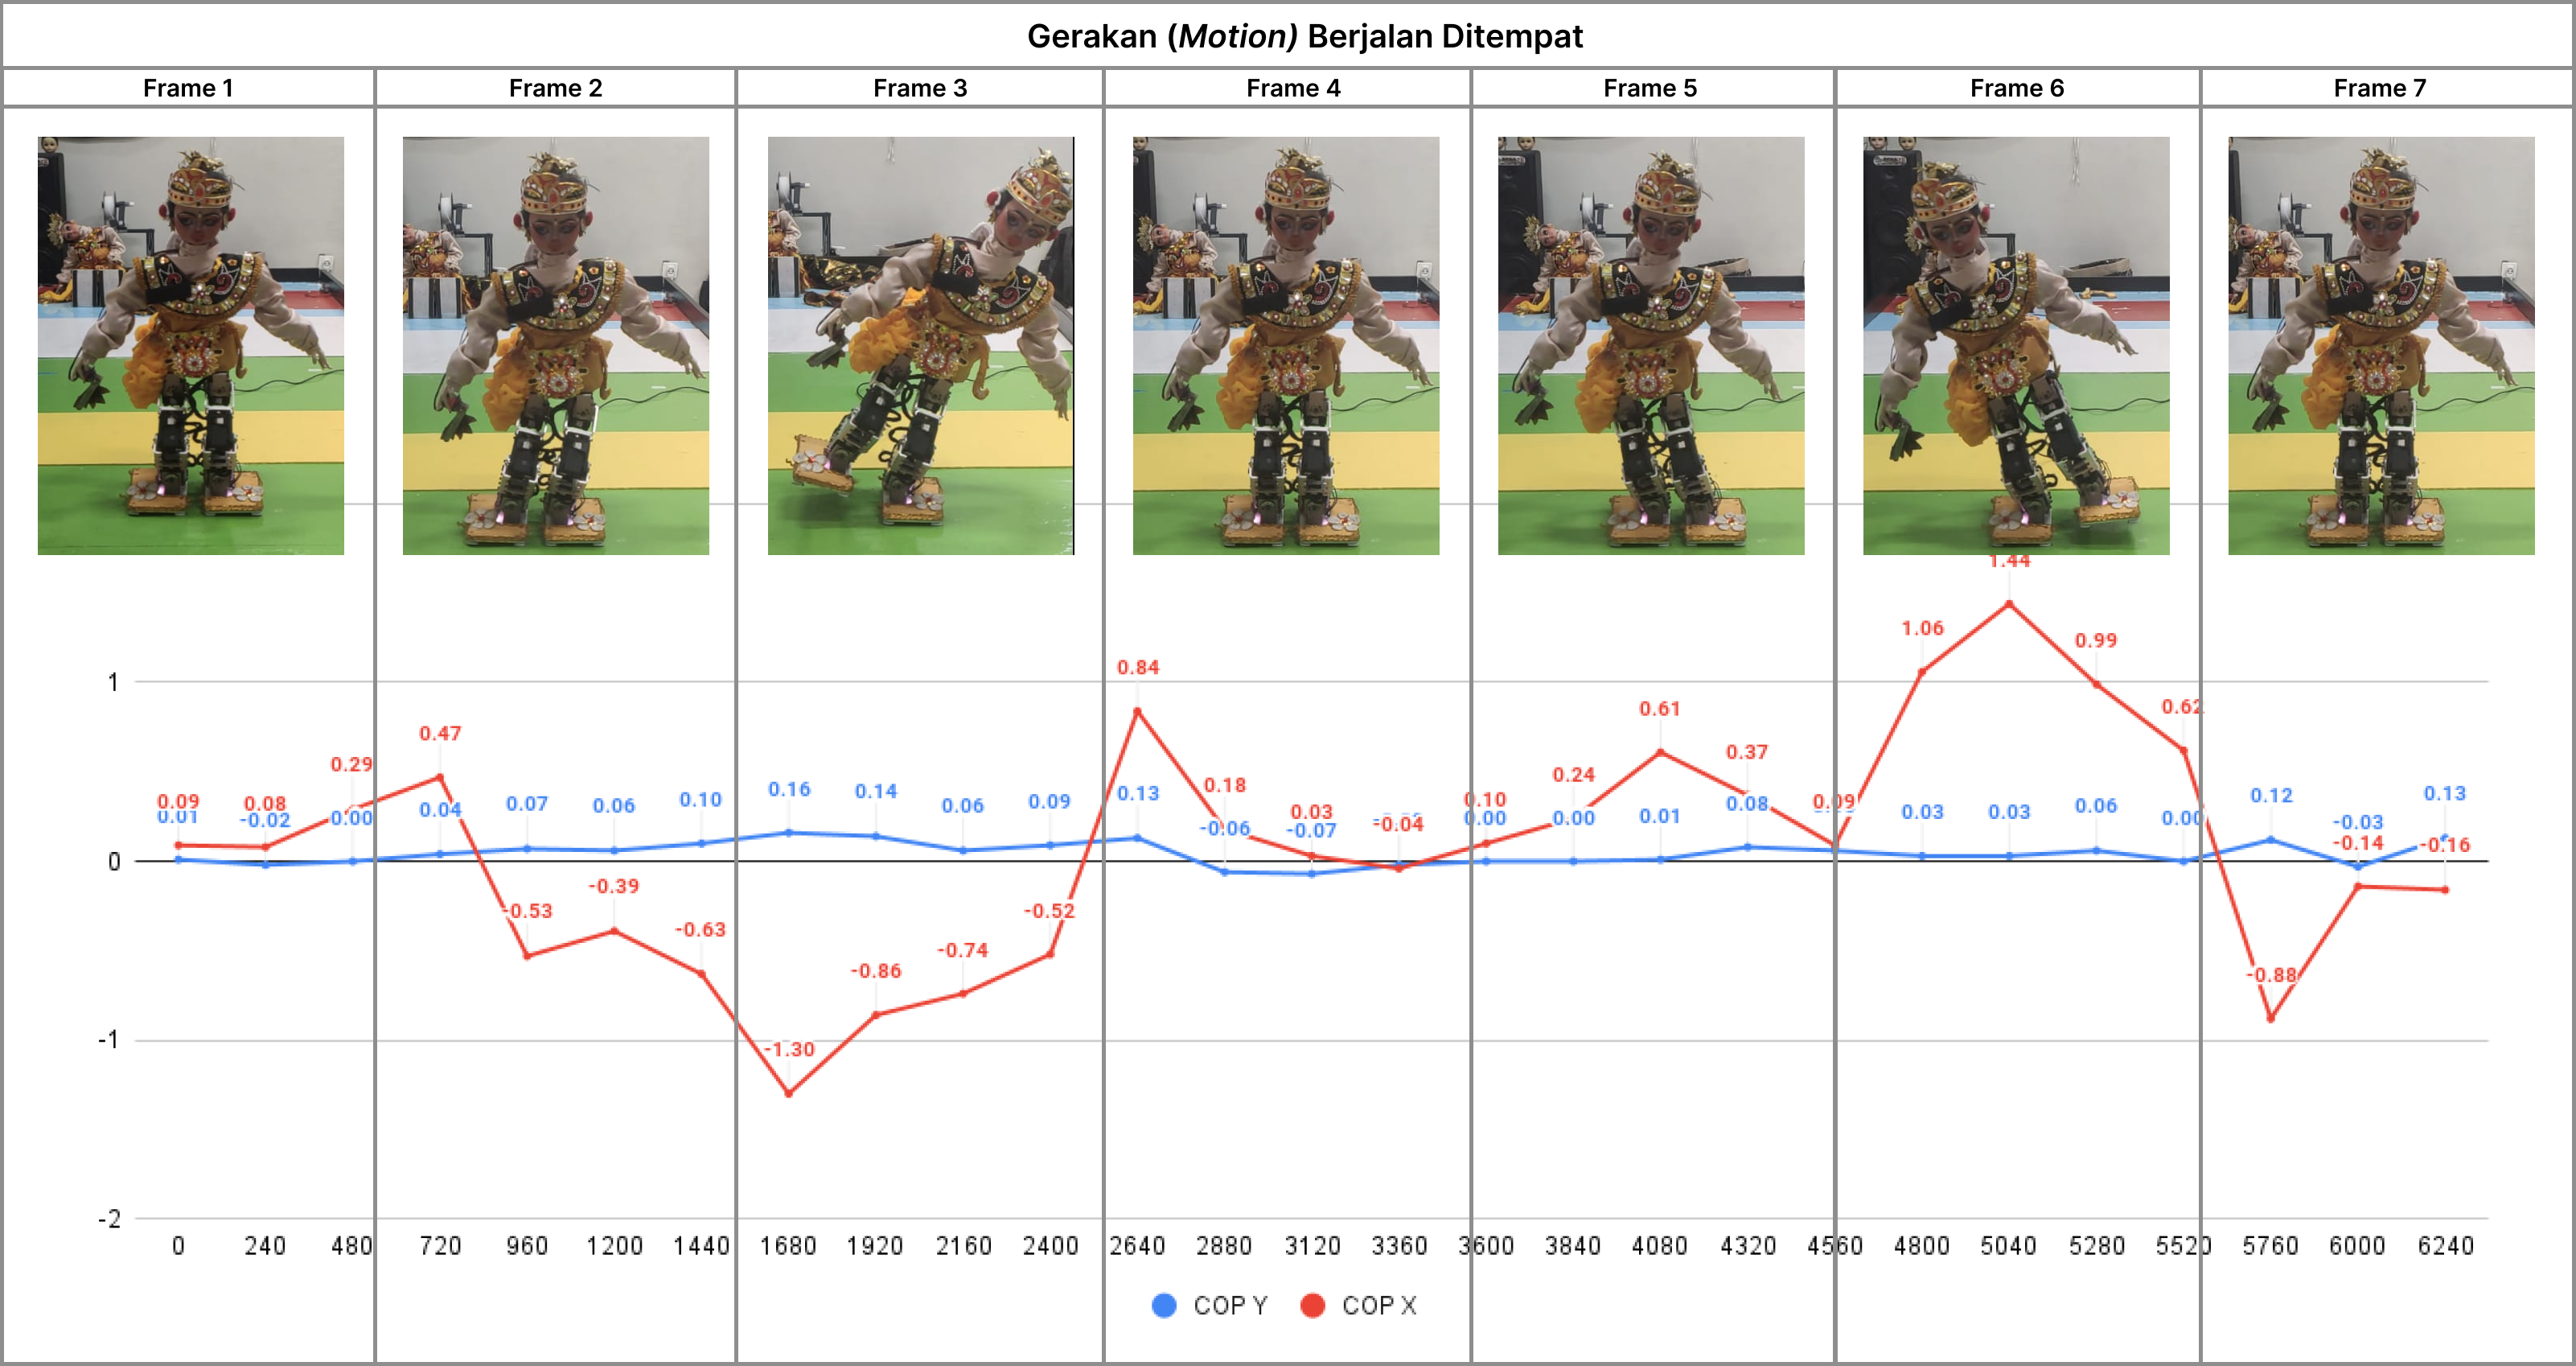
\includegraphics[width=0.45\textwidth]{gambar/motion_berjalan.png}
            \caption{Center of Pressure Graph When the Robot Walks in Place}
            \label{fig:robot_cop}
        \end{figure}

        \hspace*{1em} The test results showed that the center of pressure changes dynamically while the robot performs walking movements. When the robot lifts its right leg, the center of pressure shifts to the left leg, and the center of pressure value on the X-axis has a maximum value of 1.44. Conversely, when the robot lifts its left leg, the center of pressure shifts to the right leg, and the center of pressure value on the X-axis has a minimum value of -1.3. On the Y-axis, the center of pressure value ranges from 0.16 to -0.06, indicating that the center of pressure is in the middle of the foot sole.

    \item PID Control System Testing
    \label{subsec:results-discussion-pid}

        \hspace*{1em} This test will compare the effect of the \(K_p\) parameter on the PID control system performance. The test is conducted by measuring the Root Mean Square (RMS) and the test results on lifting the right and left legs.

        \begin{table}[h]
            \centering
            \caption{Root Mean Square (RMS) in the Effect of P Parameter Testing}
            \begin{tabular}{|c|c|}
            \hline
            \textbf{PID} & \textbf{RMS Error} \\
            \hline
            $K_p = 0.00$ & 0.7598 \\
            $K_p = 0.05$ & 0.7690 \\
            $K_p = 0.10$ & 0.7779 \\
            $K_p = 0.15$ & 0.8145 \\
            $K_p = 0.20$ & 0.8870 \\
            $K_p = 0.25$ & 0.8801 \\
            \hline
            \end{tabular}
            \label{tab:rms_p}
        \end{table}

        \begin{table}[h]
            \centering
            \caption{Test Results of the Effect of P Parameter on PID Controller, Right Leg Lifting Movement}
            \begin{tabular}{|c|c|c|c|}
                \hline
                \textbf{PID} & \textbf{Fall} & \textbf{Not Fall} & \textbf{Success} \\
                \hline
                $K_p = 0.00$ & 6 & 0 & 0   \% \\
                $K_p = 0.05$ & 6 & 0 & 0   \% \\
                $K_p = 0.10$ & 0 & 6 & 100 \% \\
                $K_p = 0.15$ & 1 & 5 & 83  \% \\
                $K_p = 0.20$ & 0 & 6 & 100 \% \\
                $K_p = 0.25$ & 2 & 4 & 66  \% \\            
                \hline
            \end{tabular}
            \label{tab:testing_p_right}
        \end{table}

        \begin{table}[h]
            \centering
            \caption{Test Results of the Effect of P Parameter on PID Controller, Left Leg Lifting Movement}
            \begin{tabular}{|c|c|c|c|}
                \hline
                \textbf{PID} & \textbf{Fall} & \textbf{Not Fall} & \textbf{Success} \\
                \hline
                $K_p = 0.00$ & 6 & 0 & 0   \% \\
                $K_p = 0.05$ & 6 & 0 & 0   \% \\
                $K_p = 0.10$ & 0 & 6 & 100 \% \\
                $K_p = 0.15$ & 1 & 5 & 83  \% \\
                $K_p = 0.20$ & 1 & 5 & 83  \% \\
                $K_p = 0.25$ & 0 & 6 & 100 \% \\            
                \hline
            \end{tabular}
            \label{tab:testing_p_left}
        \end{table}

        \hspace*{1em} From the test results presented in the tables, the optimal value of the \(K_p\) parameter that allows the robot to maintain balance well ranges from 0.10 to 0.20. At \(K_p\) = 0.00 and \(K_p\) = 0.05, all tests failed with the robot always falling, indicating that the PID control is ineffective at those values. Conversely, the \(K_p\) value of 0.10 shows the best performance with a 100\% success rate in maintaining the robot's balance during right and left leg lifting movements on a 3-degree slope.

        \hspace*{1em} Then, from the Root Mean Square (RMS) results presented in Table \ref{tab:rms_p}, it can be seen that the smallest RMS value is obtained at \(K_p\) = 0.10, indicating the least inaccuracy in the system at this value.

\end{enumerate}

% Ubah judul dan label berikut sesuai dengan yang diinginkan.
\section{Conclusion}
\label{sec:conclusion}

In this final project, the development of a balance system based on load cells for humanoid robots, specifically the VI-ROSE ITS humanoid robot, is proposed. This balance system uses four load cells on each robot's sole to detect the position of the center of pressure on the robot's sole. The position of this center of pressure is then used to control the humanoid robot's movements so that it can stand and walk stably.

% Acknowledgment jika ada
% \section{Acknowledgement}
% \label{sec:acknowledgement}

% The authors would like to thank the Ministry of Research, Technology, and Higher Education of the Republic of Indonesia for \lipsum[1]

% Menambahkan semua entri dari pustaka tanpa perlu sitasi dalam teks
\nocite{*}

% Menampilkan daftar pustaka dengan format IEEE
\bibliographystyle{IEEEtranN}
\bibliography{pustaka/pustaka.bib}

% Menyeimbangkan bagian akhir di kedua kolom
\balance

\end{document}
